% CVPR 2027 submission (review version). Built with Tectonic; tables and numbers come from make_q1_tables.py.
\documentclass[10pt,twocolumn,letterpaper]{article}

\usepackage[review]{cvpr}      % review version: anonymous, line numbers

% CVPR version: loaded after cvpr.sty, which already loads natbib, times, graphicx, amsmath, amssymb, booktabs,
% xcolor, caption and subcaption

% XeTeX (Tectonic) has no Type-1 Times: TeX Gyre Termes is the same typeface
\usepackage{fontspec}
\setmainfont{texgyretermes}[Extension=.otf, UprightFont=*-regular, BoldFont=*-bold,
  ItalicFont=*-italic, BoldItalicFont=*-bolditalic]
\setsansfont{texgyreheros}[Extension=.otf, UprightFont=*-regular, BoldFont=*-bold,
  ItalicFont=*-italic, BoldItalicFont=*-bolditalic]

\usepackage{amsfonts}
\usepackage{amsthm}
\usepackage{multirow}
\usepackage{array}
\usepackage{tikz}
\usetikzlibrary{arrows.meta,positioning,fit,calc}

\newcommand{\red}[1]{{\color{red}#1}}
\newcommand{\TODO}[1]{\textbf{\color{red}[TODO: #1]}}

% generated by make_numbers.py from results/puformer_chikusei_x4_v3/paper_analysis/q2n.json
\newcommand{\QtwonVthree}{0.9931}
\newcommand{\QtwonExactUV}{0.9988}
\newcommand{\QtwonExactUVNIR}{0.9998}
\newcommand{\RelErrUV}{0.41}
\newcommand{\RelErrMaxOther}{0.040}
\newcommand{\OracleBicA}{61.6}
\newcommand{\OracleLinA}{57.5}
\newcommand{\OracleModelA}{51.8}
\newcommand{\DefTen}{25\%}
\newcommand{\DefFifty}{75\%}
\newcommand{\CalibPsnrHi}{58.20}
\newcommand{\CalibQHi}{0.9931}
\newcommand{\CalibPsnrMid}{52.15}
\newcommand{\CalibQMid}{0.9904}

% generated by make_tables.py - do not edit
\makeatletter
\@namedef{pav@S-PSNR}{50.63}
\@namedef{pav@S-PSNR_psrt}{50.22}
\@namedef{pav@S-MPSNR_peak1}{51.11}
\@namedef{pav@S-SSIM}{0.9970}
\@namedef{pav@S-SSIM_psrt}{0.9974}
\@namedef{pav@S-SAM}{1.895}
\@namedef{pav@S-ERGAS}{0.621}
\@namedef{pav@S-RMSE_DN}{23.7}
\@namedef{pav@S-CC}{0.9994}
\@namedef{pav@S-SCC}{0.9995}
\@namedef{pav@S-Q2n}{0.9751}
\@namedef{pav@E-PSNR}{50.69}
\@namedef{pav@E-PSNR_psrt}{50.28}
\@namedef{pav@E-MPSNR_peak1}{51.17}
\@namedef{pav@E-SSIM}{0.9970}
\@namedef{pav@E-SSIM_psrt}{0.9974}
\@namedef{pav@E-SAM}{1.883}
\@namedef{pav@E-ERGAS}{0.617}
\@namedef{pav@E-RMSE_DN}{23.5}
\@namedef{pav@E-CC}{0.9994}
\@namedef{pav@E-SCC}{0.9995}
\@namedef{pav@E-Q2n}{0.9753}
\@namedef{pav@rank-PSNR}{1}
\@namedef{pav@tipbest-PSNR}{47.1597}
\@namedef{pav@tipbestname-PSNR}{Two-stage diffusion}
\@namedef{pav@rank-SSIM}{1}
\@namedef{pav@tipbest-SSIM}{0.9972}
\@namedef{pav@tipbestname-SSIM}{SMGU}
\@namedef{pav@rank-SAM}{13}
\@namedef{pav@tipbest-SAM}{1.4542}
\@namedef{pav@tipbestname-SAM}{Two-stage diffusion}
\@namedef{pav@rank-ERGAS}{1}
\@namedef{pav@tipbest-ERGAS}{0.8262}
\@namedef{pav@tipbestname-ERGAS}{Two-stage diffusion}
\@namedef{pav@rank-Q2n}{16}
\@namedef{pav@tipbest-Q2n}{0.9987}
\@namedef{pav@tipbestname-Q2n}{OTPNet}
\@namedef{pav@rank-CC}{1}
\@namedef{pav@tipbest-CC}{0.9985}
\@namedef{pav@tipbestname-CC}{Two-stage diffusion}
\@namedef{pav@rank-SCC}{1}
\@namedef{pav@tipbest-SCC}{0.9976}
\@namedef{pav@tipbestname-SCC}{Two-stage diffusion}
\@namedef{pav@rank-RMSE_DN}{1}
\@namedef{pav@tipbest-RMSE_DN}{35.71}
\@namedef{pav@tipbestname-RMSE_DN}{Two-stage diffusion}
\@namedef{pav@first}{6}
\@namedef{pav@firstlist}{PSNR, SSIM, ERGAS, CC, SCC, RMSE_DN}
\@namedef{pav@gain-PSNR}{3.53}
\@namedef{pav@red-RMSE_DN}{34.1}
\@namedef{pav@red-ERGAS}{25.3}
\@namedef{pav@red-SAM}{-29.5}
\@namedef{pav@cons-H}{79.9}
\@namedef{pav@cons-M}{77.6}
\@namedef{pav@gsa-PSNR}{34.78}
\@namedef{pav@gsa-SAM}{5.23}
\@namedef{pav@tipgsa-PSNR}{35.35}
\@namedef{pav@gsa-gap}{0.57}
\@namedef{pav@bic-PSNR}{25.52}
\@namedef{pav@iters}{93{,}850}
\@namedef{pav@hours}{10.2}
\@namedef{pav@params}{9.99}
\@namedef{pav@patches}{1.50}
\@namedef{pav@best-it}{43{,}000}
\@namedef{pav@best-val}{48.58}
\@namedef{pav@test-peak}{50.66}
\@namedef{pav@test-peak-it}{25{,}000}
\@namedef{pav@test-at-best}{50.63}
\@namedef{pav@test-end}{50.58}
\@namedef{pav@infer}{0.18}
\@namedef{pav@visual-tile}{3}
\@namedef{pav@blur-fixed-loss-min}{3.3}
\@namedef{pav@blur-fixed-loss-max}{6.8}
\@namedef{pav@blur-swap-loss-max}{0.11}
\@namedef{pav@srf-swap-delta}{-0.2}
\@namedef{pav@noise40-margin}{12.8}
\@namedef{pav@noise35-margin}{9.8}
\@namedef{pav@noise30-margin}{6.0}
\@namedef{pav@q2n}{0.9753}
\@namedef{pav@q2n-def10}{96\%}
\@namedef{pav@q2n-def50}{99\%}
\@namedef{pav@q2n-relmax}{0.561}
\@namedef{pav@q2n-relmin}{0.256}
\@namedef{pav@calib-psnr-hi}{50.69}
\@namedef{pav@calib-q-hi}{0.9753}
\@namedef{pav@calib-psnr-mid}{44.32}
\@namedef{pav@calib-q-mid}{0.9724}
\@namedef{pav@water-1}{11}
\@namedef{pav@water-2}{63}
\@namedef{pav@water-3}{7}
\@namedef{pav@water-4}{13}
\@namedef{pav@sam-water}{2.95}
\@namedef{pav@sam-nowater}{1.56}
\@namedef{pav@sam-nowater-2}{1.41}
\@namedef{pav@sam-dark10}{34}
\@namedef{pav@gsa-sam-water}{6.98}
\@namedef{pav@gsa-sam-nowater}{4.70}
\@namedef{pav@gsa-sam-nowater-2}{3.62}
\@namedef{pav@gsa-sam-dark10}{27}
\@namedef{pav@noise-floor}{1.01}
\@namedef{pav@noise-floor-2}{1.65}
\@namedef{pav@noise-floor-dark}{3.8}
\@namedef{pav@noise-floor-bright}{0.23}
\@namedef{pav@zero-pixels}{0}
\makeatother

\newcommand{\pav}[1]{\ifcsname pav@#1\endcsname\csname pav@#1\endcsname\else\textbf{??#1??}\fi}
\IfFileExists{tables/q1_numbers.tex}{% generated by make_q1_tables.py - do not edit
\expandafter\def\csname qone@abl-conv-absdelta\endcsname{0.02}
\expandafter\def\csname qone@abl-conv-consH\endcsname{78.5}
\expandafter\def\csname qone@abl-conv-consM\endcsname{73.9}
\expandafter\def\csname qone@abl-conv-delta\endcsname{-0.02}
\expandafter\def\csname qone@abl-conv-params\endcsname{9.94}
\expandafter\def\csname qone@abl-conv-psnr\endcsname{50.60}
\expandafter\def\csname qone@abl-conv-row\endcsname{j}
\expandafter\def\csname qone@abl-conv-sam\endcsname{1.909}
\expandafter\def\csname qone@abl-full-consH\endcsname{77.6}
\expandafter\def\csname qone@abl-full-consM\endcsname{74.8}
\expandafter\def\csname qone@abl-full-fixed\endcsname{43.13}
\expandafter\def\csname qone@abl-full-fixedloss\endcsname{7.50}
\expandafter\def\csname qone@abl-full-mean\endcsname{50.62}
\expandafter\def\csname qone@abl-full-nseeds\endcsname{3}
\expandafter\def\csname qone@abl-full-params\endcsname{9.99}
\expandafter\def\csname qone@abl-full-psnr\endcsname{50.63}
\expandafter\def\csname qone@abl-full-row\endcsname{a}
\expandafter\def\csname qone@abl-full-sam\endcsname{1.897}
\expandafter\def\csname qone@abl-full-std\endcsname{0.02}
\expandafter\def\csname qone@abl-full-swap\endcsname{50.50}
\expandafter\def\csname qone@abl-full-swaploss\endcsname{0.13}
\expandafter\def\csname qone@abl-k1-absdelta\endcsname{0.02}
\expandafter\def\csname qone@abl-k1-consH\endcsname{71.3}
\expandafter\def\csname qone@abl-k1-consM\endcsname{70.8}
\expandafter\def\csname qone@abl-k1-delta\endcsname{-0.02}
\expandafter\def\csname qone@abl-k1-params\endcsname{3.33}
\expandafter\def\csname qone@abl-k1-psnr\endcsname{50.60}
\expandafter\def\csname qone@abl-k1-row\endcsname{g}
\expandafter\def\csname qone@abl-k1-sam\endcsname{1.909}
\expandafter\def\csname qone@abl-k2-absdelta\endcsname{0.02}
\expandafter\def\csname qone@abl-k2-consH\endcsname{75.0}
\expandafter\def\csname qone@abl-k2-consM\endcsname{73.4}
\expandafter\def\csname qone@abl-k2-delta\endcsname{+0.02}
\expandafter\def\csname qone@abl-k2-params\endcsname{6.66}
\expandafter\def\csname qone@abl-k2-psnr\endcsname{50.64}
\expandafter\def\csname qone@abl-k2-row\endcsname{h}
\expandafter\def\csname qone@abl-k2-sam\endcsname{1.901}
\expandafter\def\csname qone@abl-k4-absdelta\endcsname{0.06}
\expandafter\def\csname qone@abl-k4-consH\endcsname{80.2}
\expandafter\def\csname qone@abl-k4-consM\endcsname{76.3}
\expandafter\def\csname qone@abl-k4-delta\endcsname{+0.06}
\expandafter\def\csname qone@abl-k4-params\endcsname{13.32}
\expandafter\def\csname qone@abl-k4-psnr\endcsname{50.68}
\expandafter\def\csname qone@abl-k4-row\endcsname{i}
\expandafter\def\csname qone@abl-k4-sam\endcsname{1.894}
\expandafter\def\csname qone@abl-l1-absdelta\endcsname{0.03}
\expandafter\def\csname qone@abl-l1-consH\endcsname{77.5}
\expandafter\def\csname qone@abl-l1-consM\endcsname{75.7}
\expandafter\def\csname qone@abl-l1-delta\endcsname{+0.03}
\expandafter\def\csname qone@abl-l1-params\endcsname{9.99}
\expandafter\def\csname qone@abl-l1-psnr\endcsname{50.66}
\expandafter\def\csname qone@abl-l1-row\endcsname{l}
\expandafter\def\csname qone@abl-l1-sam\endcsname{1.897}
\expandafter\def\csname qone@abl-learned-absdelta\endcsname{0.06}
\expandafter\def\csname qone@abl-learned-consH\endcsname{73.6}
\expandafter\def\csname qone@abl-learned-consM\endcsname{72.6}
\expandafter\def\csname qone@abl-learned-delta\endcsname{-0.06}
\expandafter\def\csname qone@abl-learned-fixed\endcsname{49.33}
\expandafter\def\csname qone@abl-learned-fixedloss\endcsname{1.24}
\expandafter\def\csname qone@abl-learned-params\endcsname{9.99}
\expandafter\def\csname qone@abl-learned-psnr\endcsname{50.57}
\expandafter\def\csname qone@abl-learned-row\endcsname{e}
\expandafter\def\csname qone@abl-learned-sam\endcsname{1.908}
\expandafter\def\csname qone@abl-nodeep-absdelta\endcsname{0.12}
\expandafter\def\csname qone@abl-nodeep-consH\endcsname{77.7}
\expandafter\def\csname qone@abl-nodeep-consM\endcsname{74.6}
\expandafter\def\csname qone@abl-nodeep-delta\endcsname{-0.12}
\expandafter\def\csname qone@abl-nodeep-params\endcsname{9.99}
\expandafter\def\csname qone@abl-nodeep-psnr\endcsname{50.50}
\expandafter\def\csname qone@abl-nodeep-row\endcsname{m}
\expandafter\def\csname qone@abl-nodeep-sam\endcsname{1.900}
\expandafter\def\csname qone@abl-nomem-absdelta\endcsname{0.05}
\expandafter\def\csname qone@abl-nomem-consH\endcsname{77.2}
\expandafter\def\csname qone@abl-nomem-consM\endcsname{74.8}
\expandafter\def\csname qone@abl-nomem-delta\endcsname{+0.05}
\expandafter\def\csname qone@abl-nomem-params\endcsname{9.98}
\expandafter\def\csname qone@abl-nomem-psnr\endcsname{50.67}
\expandafter\def\csname qone@abl-nomem-row\endcsname{f}
\expandafter\def\csname qone@abl-nomem-sam\endcsname{1.898}
\expandafter\def\csname qone@abl-nophys-absdelta\endcsname{0.17}
\expandafter\def\csname qone@abl-nophys-consH\endcsname{68.9}
\expandafter\def\csname qone@abl-nophys-consM\endcsname{73.3}
\expandafter\def\csname qone@abl-nophys-delta\endcsname{-0.17}
\expandafter\def\csname qone@abl-nophys-params\endcsname{9.99}
\expandafter\def\csname qone@abl-nophys-psnr\endcsname{50.46}
\expandafter\def\csname qone@abl-nophys-row\endcsname{b}
\expandafter\def\csname qone@abl-nophys-sam\endcsname{1.928}
\expandafter\def\csname qone@abl-nores-absdelta\endcsname{0.01}
\expandafter\def\csname qone@abl-nores-consH\endcsname{75.7}
\expandafter\def\csname qone@abl-nores-consM\endcsname{73.8}
\expandafter\def\csname qone@abl-nores-delta\endcsname{-0.01}
\expandafter\def\csname qone@abl-nores-params\endcsname{9.99}
\expandafter\def\csname qone@abl-nores-psnr\endcsname{50.62}
\expandafter\def\csname qone@abl-nores-row\endcsname{c}
\expandafter\def\csname qone@abl-nores-sam\endcsname{1.900}
\expandafter\def\csname qone@abl-seed-gain\endcsname{0.08}
\expandafter\def\csname qone@abl-window-absdelta\endcsname{0.01}
\expandafter\def\csname qone@abl-window-consH\endcsname{78.6}
\expandafter\def\csname qone@abl-window-consM\endcsname{75.5}
\expandafter\def\csname qone@abl-window-delta\endcsname{+0.01}
\expandafter\def\csname qone@abl-window-params\endcsname{9.99}
\expandafter\def\csname qone@abl-window-psnr\endcsname{50.63}
\expandafter\def\csname qone@abl-window-row\endcsname{k}
\expandafter\def\csname qone@abl-window-sam\endcsname{1.898}
\expandafter\def\csname qone@abl-zeros-absdelta\endcsname{0.08}
\expandafter\def\csname qone@abl-zeros-consH\endcsname{74.5}
\expandafter\def\csname qone@abl-zeros-consM\endcsname{73.0}
\expandafter\def\csname qone@abl-zeros-delta\endcsname{-0.08}
\expandafter\def\csname qone@abl-zeros-fixed\endcsname{46.55}
\expandafter\def\csname qone@abl-zeros-fixedloss\endcsname{3.97}
\expandafter\def\csname qone@abl-zeros-mean\endcsname{50.54}
\expandafter\def\csname qone@abl-zeros-nseeds\endcsname{3}
\expandafter\def\csname qone@abl-zeros-params\endcsname{9.99}
\expandafter\def\csname qone@abl-zeros-psnr\endcsname{50.52}
\expandafter\def\csname qone@abl-zeros-row\endcsname{d}
\expandafter\def\csname qone@abl-zeros-sam\endcsname{1.915}
\expandafter\def\csname qone@abl-zeros-std\endcsname{0.03}
\expandafter\def\csname qone@abl-zeros-swap\endcsname{49.64}
\expandafter\def\csname qone@abl-zeros-swaploss\endcsname{0.88}
\expandafter\def\csname qone@altloss-max\endcsname{3.4}
\expandafter\def\csname qone@altloss-min\endcsname{0.9}
\expandafter\def\csname qone@blind-chikusei-grid\endcsname{0.05}
\expandafter\def\csname qone@blind-chikusei-max-sigerr\endcsname{0.000}
\expandafter\def\csname qone@blind-chikusei-noisy-nominal-exact_fixed\endcsname{49.28}
\expandafter\def\csname qone@blind-chikusei-noisy-nominal-learned_fixed\endcsname{49.37}
\expandafter\def\csname qone@blind-chikusei-noisy-nominal-zeros_fixed\endcsname{49.50}
\expandafter\def\csname qone@blind-chikusei-noisy-worst-exact_estimated\endcsname{49.28}
\expandafter\def\csname qone@blind-chikusei-noisy-worst-exact_fixed\endcsname{47.58}
\expandafter\def\csname qone@blind-chikusei-noisy-worst-learned_fixed\endcsname{48.66}
\expandafter\def\csname qone@blind-chikusei-noisy-worst-zeros_estimated\endcsname{48.80}
\expandafter\def\csname qone@blind-chikusei-nominal-exact_fixed\endcsname{57.95}
\expandafter\def\csname qone@blind-chikusei-nominal-learned_fixed\endcsname{57.73}
\expandafter\def\csname qone@blind-chikusei-nominal-zeros_fixed\endcsname{57.79}
\expandafter\def\csname qone@blind-chikusei-s1.5-exact_estimated\endcsname{57.75}
\expandafter\def\csname qone@blind-chikusei-s1.5-exact_fixed\endcsname{51.41}
\expandafter\def\csname qone@blind-chikusei-s1.5-exact_oracle\endcsname{57.75}
\expandafter\def\csname qone@blind-chikusei-s1.5-learned_fixed\endcsname{54.28}
\expandafter\def\csname qone@blind-chikusei-s1.5-noise-exact_estimated\endcsname{49.38}
\expandafter\def\csname qone@blind-chikusei-s1.5-noise-exact_fixed\endcsname{47.58}
\expandafter\def\csname qone@blind-chikusei-s1.5-noise-exact_oracle\endcsname{49.38}
\expandafter\def\csname qone@blind-chikusei-s1.5-noise-learned_fixed\endcsname{48.66}
\expandafter\def\csname qone@blind-chikusei-s1.5-noise-sigerr\endcsname{0.000}
\expandafter\def\csname qone@blind-chikusei-s1.5-noise-zeros_estimated\endcsname{48.80}
\expandafter\def\csname qone@blind-chikusei-s1.5-sigerr\endcsname{0.000}
\expandafter\def\csname qone@blind-chikusei-s1.5-zeros_estimated\endcsname{54.39}
\expandafter\def\csname qone@blind-chikusei-s2-exact_estimated\endcsname{57.95}
\expandafter\def\csname qone@blind-chikusei-s2-exact_fixed\endcsname{57.95}
\expandafter\def\csname qone@blind-chikusei-s2-exact_oracle\endcsname{57.95}
\expandafter\def\csname qone@blind-chikusei-s2-learned_fixed\endcsname{57.73}
\expandafter\def\csname qone@blind-chikusei-s2-noise-exact_estimated\endcsname{49.28}
\expandafter\def\csname qone@blind-chikusei-s2-noise-exact_fixed\endcsname{49.28}
\expandafter\def\csname qone@blind-chikusei-s2-noise-exact_oracle\endcsname{49.28}
\expandafter\def\csname qone@blind-chikusei-s2-noise-learned_fixed\endcsname{49.37}
\expandafter\def\csname qone@blind-chikusei-s2-noise-sigerr\endcsname{0.000}
\expandafter\def\csname qone@blind-chikusei-s2-noise-zeros_estimated\endcsname{49.50}
\expandafter\def\csname qone@blind-chikusei-s2-sigerr\endcsname{0.000}
\expandafter\def\csname qone@blind-chikusei-s2-zeros_estimated\endcsname{57.79}
\expandafter\def\csname qone@blind-chikusei-s2.5-exact_estimated\endcsname{57.86}
\expandafter\def\csname qone@blind-chikusei-s2.5-exact_fixed\endcsname{54.59}
\expandafter\def\csname qone@blind-chikusei-s2.5-exact_oracle\endcsname{57.86}
\expandafter\def\csname qone@blind-chikusei-s2.5-learned_fixed\endcsname{56.19}
\expandafter\def\csname qone@blind-chikusei-s2.5-noise-exact_estimated\endcsname{49.36}
\expandafter\def\csname qone@blind-chikusei-s2.5-noise-exact_fixed\endcsname{48.66}
\expandafter\def\csname qone@blind-chikusei-s2.5-noise-exact_oracle\endcsname{49.36}
\expandafter\def\csname qone@blind-chikusei-s2.5-noise-learned_fixed\endcsname{49.11}
\expandafter\def\csname qone@blind-chikusei-s2.5-noise-sigerr\endcsname{0.000}
\expandafter\def\csname qone@blind-chikusei-s2.5-noise-zeros_estimated\endcsname{49.41}
\expandafter\def\csname qone@blind-chikusei-s2.5-sigerr\endcsname{0.000}
\expandafter\def\csname qone@blind-chikusei-s2.5-zeros_estimated\endcsname{56.62}
\expandafter\def\csname qone@blind-chikusei-s3-exact_estimated\endcsname{57.70}
\expandafter\def\csname qone@blind-chikusei-s3-exact_fixed\endcsname{52.32}
\expandafter\def\csname qone@blind-chikusei-s3-exact_oracle\endcsname{57.70}
\expandafter\def\csname qone@blind-chikusei-s3-learned_fixed\endcsname{54.72}
\expandafter\def\csname qone@blind-chikusei-s3-noise-exact_estimated\endcsname{49.40}
\expandafter\def\csname qone@blind-chikusei-s3-noise-exact_fixed\endcsname{47.94}
\expandafter\def\csname qone@blind-chikusei-s3-noise-exact_oracle\endcsname{49.40}
\expandafter\def\csname qone@blind-chikusei-s3-noise-learned_fixed\endcsname{48.77}
\expandafter\def\csname qone@blind-chikusei-s3-noise-sigerr\endcsname{0.000}
\expandafter\def\csname qone@blind-chikusei-s3-noise-zeros_estimated\endcsname{49.20}
\expandafter\def\csname qone@blind-chikusei-s3-sigerr\endcsname{0.000}
\expandafter\def\csname qone@blind-chikusei-s3-zeros_estimated\endcsname{55.36}
\expandafter\def\csname qone@blind-chikusei-worst-exact_estimated\endcsname{57.70}
\expandafter\def\csname qone@blind-chikusei-worst-exact_fixed\endcsname{51.41}
\expandafter\def\csname qone@blind-chikusei-worst-learned_fixed\endcsname{54.28}
\expandafter\def\csname qone@blind-chikusei-worst-zeros_estimated\endcsname{54.39}
\expandafter\def\csname qone@blind-pavia-grid\endcsname{0.05}
\expandafter\def\csname qone@blind-pavia-max-sigerr\endcsname{0.000}
\expandafter\def\csname qone@blind-pavia-noisy-nominal-exact_fixed\endcsname{44.56}
\expandafter\def\csname qone@blind-pavia-noisy-nominal-learned_fixed\endcsname{44.77}
\expandafter\def\csname qone@blind-pavia-noisy-nominal-zeros_fixed\endcsname{44.84}
\expandafter\def\csname qone@blind-pavia-noisy-worst-exact_estimated\endcsname{44.56}
\expandafter\def\csname qone@blind-pavia-noisy-worst-exact_fixed\endcsname{41.26}
\expandafter\def\csname qone@blind-pavia-noisy-worst-learned_fixed\endcsname{44.41}
\expandafter\def\csname qone@blind-pavia-noisy-worst-zeros_estimated\endcsname{44.59}
\expandafter\def\csname qone@blind-pavia-nominal-exact_fixed\endcsname{50.63}
\expandafter\def\csname qone@blind-pavia-nominal-learned_fixed\endcsname{50.57}
\expandafter\def\csname qone@blind-pavia-nominal-zeros_fixed\endcsname{50.52}
\expandafter\def\csname qone@blind-pavia-s1.5-exact_estimated\endcsname{50.54}
\expandafter\def\csname qone@blind-pavia-s1.5-exact_fixed\endcsname{43.13}
\expandafter\def\csname qone@blind-pavia-s1.5-exact_oracle\endcsname{50.54}
\expandafter\def\csname qone@blind-pavia-s1.5-learned_fixed\endcsname{49.33}
\expandafter\def\csname qone@blind-pavia-s1.5-noise-exact_estimated\endcsname{44.71}
\expandafter\def\csname qone@blind-pavia-s1.5-noise-exact_fixed\endcsname{41.26}
\expandafter\def\csname qone@blind-pavia-s1.5-noise-exact_oracle\endcsname{44.71}
\expandafter\def\csname qone@blind-pavia-s1.5-noise-learned_fixed\endcsname{44.41}
\expandafter\def\csname qone@blind-pavia-s1.5-noise-sigerr\endcsname{0.000}
\expandafter\def\csname qone@blind-pavia-s1.5-noise-zeros_estimated\endcsname{44.59}
\expandafter\def\csname qone@blind-pavia-s1.5-sigerr\endcsname{0.000}
\expandafter\def\csname qone@blind-pavia-s1.5-zeros_estimated\endcsname{49.64}
\expandafter\def\csname qone@blind-pavia-s2-exact_estimated\endcsname{50.63}
\expandafter\def\csname qone@blind-pavia-s2-exact_fixed\endcsname{50.63}
\expandafter\def\csname qone@blind-pavia-s2-exact_oracle\endcsname{50.63}
\expandafter\def\csname qone@blind-pavia-s2-learned_fixed\endcsname{50.57}
\expandafter\def\csname qone@blind-pavia-s2-noise-exact_estimated\endcsname{44.56}
\expandafter\def\csname qone@blind-pavia-s2-noise-exact_fixed\endcsname{44.56}
\expandafter\def\csname qone@blind-pavia-s2-noise-exact_oracle\endcsname{44.56}
\expandafter\def\csname qone@blind-pavia-s2-noise-learned_fixed\endcsname{44.77}
\expandafter\def\csname qone@blind-pavia-s2-noise-sigerr\endcsname{0.000}
\expandafter\def\csname qone@blind-pavia-s2-noise-zeros_estimated\endcsname{44.84}
\expandafter\def\csname qone@blind-pavia-s2-sigerr\endcsname{0.000}
\expandafter\def\csname qone@blind-pavia-s2-zeros_estimated\endcsname{50.52}
\expandafter\def\csname qone@blind-pavia-s2.5-exact_estimated\endcsname{50.58}
\expandafter\def\csname qone@blind-pavia-s2.5-exact_fixed\endcsname{46.73}
\expandafter\def\csname qone@blind-pavia-s2.5-exact_oracle\endcsname{50.58}
\expandafter\def\csname qone@blind-pavia-s2.5-learned_fixed\endcsname{49.99}
\expandafter\def\csname qone@blind-pavia-s2.5-noise-exact_estimated\endcsname{44.61}
\expandafter\def\csname qone@blind-pavia-s2.5-noise-exact_fixed\endcsname{43.23}
\expandafter\def\csname qone@blind-pavia-s2.5-noise-exact_oracle\endcsname{44.61}
\expandafter\def\csname qone@blind-pavia-s2.5-noise-learned_fixed\endcsname{44.64}
\expandafter\def\csname qone@blind-pavia-s2.5-noise-sigerr\endcsname{0.000}
\expandafter\def\csname qone@blind-pavia-s2.5-noise-zeros_estimated\endcsname{44.84}
\expandafter\def\csname qone@blind-pavia-s2.5-sigerr\endcsname{0.000}
\expandafter\def\csname qone@blind-pavia-s2.5-zeros_estimated\endcsname{50.26}
\expandafter\def\csname qone@blind-pavia-s3-exact_estimated\endcsname{50.50}
\expandafter\def\csname qone@blind-pavia-s3-exact_fixed\endcsname{44.18}
\expandafter\def\csname qone@blind-pavia-s3-exact_oracle\endcsname{50.50}
\expandafter\def\csname qone@blind-pavia-s3-learned_fixed\endcsname{49.36}
\expandafter\def\csname qone@blind-pavia-s3-noise-exact_estimated\endcsname{44.64}
\expandafter\def\csname qone@blind-pavia-s3-noise-exact_fixed\endcsname{41.90}
\expandafter\def\csname qone@blind-pavia-s3-noise-exact_oracle\endcsname{44.64}
\expandafter\def\csname qone@blind-pavia-s3-noise-learned_fixed\endcsname{44.45}
\expandafter\def\csname qone@blind-pavia-s3-noise-sigerr\endcsname{0.000}
\expandafter\def\csname qone@blind-pavia-s3-noise-zeros_estimated\endcsname{44.78}
\expandafter\def\csname qone@blind-pavia-s3-sigerr\endcsname{0.000}
\expandafter\def\csname qone@blind-pavia-s3-zeros_estimated\endcsname{49.91}
\expandafter\def\csname qone@blind-pavia-worst-exact_estimated\endcsname{50.50}
\expandafter\def\csname qone@blind-pavia-worst-exact_fixed\endcsname{43.13}
\expandafter\def\csname qone@blind-pavia-worst-learned_fixed\endcsname{49.33}
\expandafter\def\csname qone@blind-pavia-worst-zeros_estimated\endcsname{49.64}
\expandafter\def\csname qone@chikusei4-allwin\endcsname{all}
\expandafter\def\csname qone@chikusei4-best-other\endcsname{MIMFormer}
\expandafter\def\csname qone@chikusei4-bicubic-psnr\endcsname{33.63}
\expandafter\def\csname qone@chikusei4-bicubic-sam\endcsname{4.406}
\expandafter\def\csname qone@chikusei4-dct-iters\endcsname{4{,}850}
\expandafter\def\csname qone@chikusei4-dct-psnr\endcsname{53.18}
\expandafter\def\csname qone@chikusei4-dct-sam\endcsname{1.133}
\expandafter\def\csname qone@chikusei4-dhif-iters\endcsname{3{,}250}
\expandafter\def\csname qone@chikusei4-dhif-psnr\endcsname{54.39}
\expandafter\def\csname qone@chikusei4-dhif-sam\endcsname{1.020}
\expandafter\def\csname qone@chikusei4-gain\endcsname{0.99}
\expandafter\def\csname qone@chikusei4-gsa-psnr\endcsname{43.20}
\expandafter\def\csname qone@chikusei4-gsa-sam\endcsname{2.730}
\expandafter\def\csname qone@chikusei4-mimformer-iters\endcsname{100{,}000}
\expandafter\def\csname qone@chikusei4-mimformer-psnr\endcsname{56.96}
\expandafter\def\csname qone@chikusei4-mimformer-sam\endcsname{0.801}
\expandafter\def\csname qone@chikusei4-nimg\endcsname{8}
\expandafter\def\csname qone@chikusei4-p\endcsname{3.9e-03}
\expandafter\def\csname qone@chikusei4-psnr\endcsname{57.95}
\expandafter\def\csname qone@chikusei4-psrt-iters\endcsname{64{,}000}
\expandafter\def\csname qone@chikusei4-psrt-psnr\endcsname{53.99}
\expandafter\def\csname qone@chikusei4-psrt-sam\endcsname{1.057}
\expandafter\def\csname qone@chikusei4-puformer-iters\endcsname{35{,}750}
\expandafter\def\csname qone@chikusei4-puformer-psnr\endcsname{57.95}
\expandafter\def\csname qone@chikusei4-puformer-sam\endcsname{0.731}
\expandafter\def\csname qone@chikusei4-rmse-red\endcsname{10}
\expandafter\def\csname qone@chikusei4-sam\endcsname{0.731}
\expandafter\def\csname qone@chikusei4-ssrnet-iters\endcsname{300{,}000}
\expandafter\def\csname qone@chikusei4-ssrnet-psnr\endcsname{55.55}
\expandafter\def\csname qone@chikusei4-ssrnet-sam\endcsname{0.954}
\expandafter\def\csname qone@fp-chikusei-exact-crop\endcsname{0.00}
\expandafter\def\csname qone@fp-chikusei-exact-test\endcsname{0.00}
\expandafter\def\csname qone@fp-chikusei-learned-crop\endcsname{10.06}
\expandafter\def\csname qone@fp-chikusei-learned-test\endcsname{4.62}
\expandafter\def\csname qone@fp-chikusei-zeros-crop\endcsname{10.03}
\expandafter\def\csname qone@fp-chikusei-zeros-test\endcsname{4.61}
\expandafter\def\csname qone@fp-pavia-exact-crop\endcsname{0.00}
\expandafter\def\csname qone@fp-pavia-exact-test\endcsname{0.00}
\expandafter\def\csname qone@fp-pavia-learned-crop\endcsname{11.17}
\expandafter\def\csname qone@fp-pavia-learned-test\endcsname{4.69}
\expandafter\def\csname qone@fp-pavia-zeros-crop\endcsname{11.11}
\expandafter\def\csname qone@fp-pavia-zeros-test\endcsname{4.66}
\expandafter\def\csname qone@kabl-conv-absdelta\endcsname{0.07}
\expandafter\def\csname qone@kabl-conv-consH\endcsname{85.2}
\expandafter\def\csname qone@kabl-conv-consM\endcsname{85.9}
\expandafter\def\csname qone@kabl-conv-delta\endcsname{+0.07}
\expandafter\def\csname qone@kabl-conv-params\endcsname{10.09}
\expandafter\def\csname qone@kabl-conv-psnr\endcsname{58.02}
\expandafter\def\csname qone@kabl-conv-row\endcsname{w}
\expandafter\def\csname qone@kabl-conv-sam\endcsname{0.724}
\expandafter\def\csname qone@kabl-full-consH\endcsname{83.9}
\expandafter\def\csname qone@kabl-full-consM\endcsname{83.4}
\expandafter\def\csname qone@kabl-full-fixed\endcsname{51.41}
\expandafter\def\csname qone@kabl-full-fixedloss\endcsname{6.53}
\expandafter\def\csname qone@kabl-full-mean\endcsname{57.95}
\expandafter\def\csname qone@kabl-full-nseeds\endcsname{3}
\expandafter\def\csname qone@kabl-full-params\endcsname{10.13}
\expandafter\def\csname qone@kabl-full-psnr\endcsname{57.95}
\expandafter\def\csname qone@kabl-full-row\endcsname{n}
\expandafter\def\csname qone@kabl-full-sam\endcsname{0.731}
\expandafter\def\csname qone@kabl-full-std\endcsname{0.004}
\expandafter\def\csname qone@kabl-full-swap\endcsname{57.70}
\expandafter\def\csname qone@kabl-full-swaploss\endcsname{0.25}
\expandafter\def\csname qone@kabl-k1-absdelta\endcsname{0.20}
\expandafter\def\csname qone@kabl-k1-consH\endcsname{77.4}
\expandafter\def\csname qone@kabl-k1-consM\endcsname{77.1}
\expandafter\def\csname qone@kabl-k1-delta\endcsname{-0.20}
\expandafter\def\csname qone@kabl-k1-params\endcsname{3.37}
\expandafter\def\csname qone@kabl-k1-psnr\endcsname{57.75}
\expandafter\def\csname qone@kabl-k1-row\endcsname{t}
\expandafter\def\csname qone@kabl-k1-sam\endcsname{0.743}
\expandafter\def\csname qone@kabl-k2-absdelta\endcsname{0.02}
\expandafter\def\csname qone@kabl-k2-consH\endcsname{81.0}
\expandafter\def\csname qone@kabl-k2-consM\endcsname{81.6}
\expandafter\def\csname qone@kabl-k2-delta\endcsname{-0.02}
\expandafter\def\csname qone@kabl-k2-params\endcsname{6.75}
\expandafter\def\csname qone@kabl-k2-psnr\endcsname{57.92}
\expandafter\def\csname qone@kabl-k2-row\endcsname{u}
\expandafter\def\csname qone@kabl-k2-sam\endcsname{0.731}
\expandafter\def\csname qone@kabl-k4-absdelta\endcsname{0.01}
\expandafter\def\csname qone@kabl-k4-consH\endcsname{85.0}
\expandafter\def\csname qone@kabl-k4-consM\endcsname{82.7}
\expandafter\def\csname qone@kabl-k4-delta\endcsname{+0.01}
\expandafter\def\csname qone@kabl-k4-params\endcsname{13.51}
\expandafter\def\csname qone@kabl-k4-psnr\endcsname{57.96}
\expandafter\def\csname qone@kabl-k4-row\endcsname{v}
\expandafter\def\csname qone@kabl-k4-sam\endcsname{0.728}
\expandafter\def\csname qone@kabl-l1-absdelta\endcsname{0.02}
\expandafter\def\csname qone@kabl-l1-consH\endcsname{82.2}
\expandafter\def\csname qone@kabl-l1-consM\endcsname{83.0}
\expandafter\def\csname qone@kabl-l1-delta\endcsname{+0.02}
\expandafter\def\csname qone@kabl-l1-params\endcsname{10.13}
\expandafter\def\csname qone@kabl-l1-psnr\endcsname{57.97}
\expandafter\def\csname qone@kabl-l1-row\endcsname{y}
\expandafter\def\csname qone@kabl-l1-sam\endcsname{0.731}
\expandafter\def\csname qone@kabl-learned-absdelta\endcsname{0.22}
\expandafter\def\csname qone@kabl-learned-consH\endcsname{77.1}
\expandafter\def\csname qone@kabl-learned-consM\endcsname{75.3}
\expandafter\def\csname qone@kabl-learned-delta\endcsname{-0.22}
\expandafter\def\csname qone@kabl-learned-fixed\endcsname{54.28}
\expandafter\def\csname qone@kabl-learned-fixedloss\endcsname{3.45}
\expandafter\def\csname qone@kabl-learned-params\endcsname{10.13}
\expandafter\def\csname qone@kabl-learned-psnr\endcsname{57.73}
\expandafter\def\csname qone@kabl-learned-row\endcsname{r}
\expandafter\def\csname qone@kabl-learned-sam\endcsname{0.739}
\expandafter\def\csname qone@kabl-nodeep-absdelta\endcsname{0.04}
\expandafter\def\csname qone@kabl-nodeep-consH\endcsname{84.1}
\expandafter\def\csname qone@kabl-nodeep-consM\endcsname{83.7}
\expandafter\def\csname qone@kabl-nodeep-delta\endcsname{+0.04}
\expandafter\def\csname qone@kabl-nodeep-params\endcsname{10.13}
\expandafter\def\csname qone@kabl-nodeep-psnr\endcsname{57.99}
\expandafter\def\csname qone@kabl-nodeep-row\endcsname{z}
\expandafter\def\csname qone@kabl-nodeep-sam\endcsname{0.727}
\expandafter\def\csname qone@kabl-nomem-absdelta\endcsname{0.01}
\expandafter\def\csname qone@kabl-nomem-consH\endcsname{84.1}
\expandafter\def\csname qone@kabl-nomem-consM\endcsname{83.0}
\expandafter\def\csname qone@kabl-nomem-delta\endcsname{+0.01}
\expandafter\def\csname qone@kabl-nomem-params\endcsname{10.12}
\expandafter\def\csname qone@kabl-nomem-psnr\endcsname{57.96}
\expandafter\def\csname qone@kabl-nomem-row\endcsname{s}
\expandafter\def\csname qone@kabl-nomem-sam\endcsname{0.728}
\expandafter\def\csname qone@kabl-nophys-absdelta\endcsname{0.30}
\expandafter\def\csname qone@kabl-nophys-consH\endcsname{73.3}
\expandafter\def\csname qone@kabl-nophys-consM\endcsname{73.7}
\expandafter\def\csname qone@kabl-nophys-delta\endcsname{-0.30}
\expandafter\def\csname qone@kabl-nophys-params\endcsname{10.13}
\expandafter\def\csname qone@kabl-nophys-psnr\endcsname{57.65}
\expandafter\def\csname qone@kabl-nophys-row\endcsname{o}
\expandafter\def\csname qone@kabl-nophys-sam\endcsname{0.752}
\expandafter\def\csname qone@kabl-nores-absdelta\endcsname{0.06}
\expandafter\def\csname qone@kabl-nores-consH\endcsname{82.8}
\expandafter\def\csname qone@kabl-nores-consM\endcsname{82.8}
\expandafter\def\csname qone@kabl-nores-delta\endcsname{+0.06}
\expandafter\def\csname qone@kabl-nores-params\endcsname{10.13}
\expandafter\def\csname qone@kabl-nores-psnr\endcsname{58.01}
\expandafter\def\csname qone@kabl-nores-row\endcsname{p}
\expandafter\def\csname qone@kabl-nores-sam\endcsname{0.727}
\expandafter\def\csname qone@kabl-seed-gain\endcsname{0.22}
\expandafter\def\csname qone@kabl-window-absdelta\endcsname{0.03}
\expandafter\def\csname qone@kabl-window-consH\endcsname{84.4}
\expandafter\def\csname qone@kabl-window-consM\endcsname{85.0}
\expandafter\def\csname qone@kabl-window-delta\endcsname{+0.03}
\expandafter\def\csname qone@kabl-window-params\endcsname{10.13}
\expandafter\def\csname qone@kabl-window-psnr\endcsname{57.98}
\expandafter\def\csname qone@kabl-window-row\endcsname{x}
\expandafter\def\csname qone@kabl-window-sam\endcsname{0.725}
\expandafter\def\csname qone@kabl-zeros-absdelta\endcsname{0.22}
\expandafter\def\csname qone@kabl-zeros-consH\endcsname{75.9}
\expandafter\def\csname qone@kabl-zeros-consM\endcsname{74.4}
\expandafter\def\csname qone@kabl-zeros-delta\endcsname{-0.22}
\expandafter\def\csname qone@kabl-zeros-fixed\endcsname{53.06}
\expandafter\def\csname qone@kabl-zeros-fixedloss\endcsname{4.73}
\expandafter\def\csname qone@kabl-zeros-mean\endcsname{57.73}
\expandafter\def\csname qone@kabl-zeros-nseeds\endcsname{3}
\expandafter\def\csname qone@kabl-zeros-params\endcsname{10.13}
\expandafter\def\csname qone@kabl-zeros-psnr\endcsname{57.79}
\expandafter\def\csname qone@kabl-zeros-row\endcsname{q}
\expandafter\def\csname qone@kabl-zeros-sam\endcsname{0.738}
\expandafter\def\csname qone@kabl-zeros-std\endcsname{0.05}
\expandafter\def\csname qone@kabl-zeros-swap\endcsname{54.38}
\expandafter\def\csname qone@kabl-zeros-swaploss\endcsname{3.41}
\expandafter\def\csname qone@long-gap\endcsname{0.69}
\expandafter\def\csname qone@long-mimformer-iters\endcsname{194{,}950}
\expandafter\def\csname qone@long-mimformer-psnr\endcsname{49.97}
\expandafter\def\csname qone@long-puformer-iters\endcsname{79{,}050}
\expandafter\def\csname qone@long-puformer-psnr\endcsname{50.67}
\expandafter\def\csname qone@pavia4-allwin\endcsname{all}
\expandafter\def\csname qone@pavia4-best-other\endcsname{MIMFormer}
\expandafter\def\csname qone@pavia4-bicubic-psnr\endcsname{25.52}
\expandafter\def\csname qone@pavia4-bicubic-sam\endcsname{6.554}
\expandafter\def\csname qone@pavia4-dct-iters\endcsname{4{,}800}
\expandafter\def\csname qone@pavia4-dct-psnr\endcsname{46.94}
\expandafter\def\csname qone@pavia4-dct-sam\endcsname{2.442}
\expandafter\def\csname qone@pavia4-dhif-iters\endcsname{3{,}950}
\expandafter\def\csname qone@pavia4-dhif-psnr\endcsname{47.67}
\expandafter\def\csname qone@pavia4-dhif-sam\endcsname{2.295}
\expandafter\def\csname qone@pavia4-gain\endcsname{1.00}
\expandafter\def\csname qone@pavia4-gsa-psnr\endcsname{34.78}
\expandafter\def\csname qone@pavia4-gsa-sam\endcsname{5.229}
\expandafter\def\csname qone@pavia4-mimformer-iters\endcsname{97{,}400}
\expandafter\def\csname qone@pavia4-mimformer-psnr\endcsname{49.63}
\expandafter\def\csname qone@pavia4-mimformer-sam\endcsname{1.982}
\expandafter\def\csname qone@pavia4-nimg\endcsname{4}
\expandafter\def\csname qone@pavia4-p\endcsname{--}
\expandafter\def\csname qone@pavia4-psnr\endcsname{50.63}
\expandafter\def\csname qone@pavia4-psrt-iters\endcsname{65{,}200}
\expandafter\def\csname qone@pavia4-psrt-psnr\endcsname{47.87}
\expandafter\def\csname qone@pavia4-psrt-sam\endcsname{2.212}
\expandafter\def\csname qone@pavia4-puformer-iters\endcsname{37{,}450}
\expandafter\def\csname qone@pavia4-puformer-psnr\endcsname{50.63}
\expandafter\def\csname qone@pavia4-puformer-sam\endcsname{1.897}
\expandafter\def\csname qone@pavia4-rmse-red\endcsname{11}
\expandafter\def\csname qone@pavia4-sam\endcsname{1.897}
\expandafter\def\csname qone@pavia4-ssrnet-iters\endcsname{300{,}000}
\expandafter\def\csname qone@pavia4-ssrnet-psnr\endcsname{48.45}
\expandafter\def\csname qone@pavia4-ssrnet-sam\endcsname{2.443}
\expandafter\def\csname qone@settings-allwin\endcsname{2}
\expandafter\def\csname qone@settings-done\endcsname{2}
\expandafter\def\csname qone@settings-total\endcsname{2}
\expandafter\def\csname qone@swaploss-max\endcsname{0.25}
\expandafter\def\csname qone@swaploss-n\endcsname{2}
\expandafter\def\csname qone@wins-ERGAS\endcsname{2}
\expandafter\def\csname qone@wins-PSNR\endcsname{2}
\expandafter\def\csname qone@wins-SAM\endcsname{2}
}{}
\newcommand{\qone}[1]{\ifcsname qone@#1\endcsname\csname qone@#1\endcsname\else\textbf{??}\fi}
\newcommand{\qtab}[1]{\IfFileExists{tables/#1.tex}{\input{tables/#1.tex}}{}}

\newtheorem{theorem}{Theorem}
\newtheorem{proposition}{Proposition}
\newtheorem{corollary}{Corollary}

\newcommand{\best}[1]{\textbf{#1}}
\newcommand{\bm}[1]{\boldsymbol{#1}}
\newcommand{\X}{\mathbf{X}}
\newcommand{\Z}{\mathbf{Z}}
\newcommand{\YH}{\mathbf{Y}_{\mathrm{H}}}
\newcommand{\YM}{\mathbf{Y}_{\mathrm{M}}}
\newcommand{\D}{\mathcal{D}}
\newcommand{\R}{\mathcal{R}}
\newcommand{\supp}{the supplementary material}


\definecolor{cvprblue}{rgb}{0.21,0.49,0.74}
\usepackage[pagebackref,breaklinks,colorlinks,allcolors=cvprblue]{hyperref}

\def\confName{CVPR}
\def\confYear{2027}

\title{Unfolded Hyperspectral and Multispectral Image Fusion with Exact Observation Operators}

\author{Anonymous CVPR submission}

\begin{document}
\maketitle

\begin{abstract}
Deep unfolding networks for hyperspectral and multispectral image fusion alternate data-consistency steps with learned priors. In most of them the blur, downsampling and spectral-response operators are learned or use zero padding, so they differ from the operators that produced the data, and each network is trained for a single sensor pair. We study what exact operators bring to such a network. With a separable blur and the true border rule, the data step has a closed form in a product eigenbasis, and the null space of fusion, the part of the image that no observation constrains, is explicit. An exact data step keeps the ground truth fixed, while an inexact one moves it by an amount that we bound, and both operators can be estimated from the two observations. Our network, PUFormer, combines exact data steps with a residual U-Net prior and is trained over a family of blurs, spectral responses and noise levels. We retrain \qone{n-retrained-word} published fusion networks from their authors' code under one protocol and training budget. PUFormer is the most accurate on Chikusei and Pavia Centre, by \qone{chikusei4-gain} and \qone{pavia4-gain}~dB PSNR, and its error in the observed subspace is \qone{null-pavia-obs-ratio}--\qone{null-chikusei-obs-ratio} times smaller. Most of the margin comes from the prior and its training; the exact data steps add a smaller gain and make the operator replaceable at test time. Trained over the operator family, PUFormer stays accurate when the blur, the spectral response or the noise change, but not under misregistration.
\end{abstract}

\section{Introduction}
\label{sec:intro}
Hyperspectral cameras record hundreds of narrow bands at a coarse spatial resolution, and multispectral cameras record a few broad bands at a fine one. Fusing the two images gives a high-resolution hyperspectral image (HR-HSI)~\cite{yokoya2017review,vivone2025deep}. Most recent methods are deep networks trained on simulated pairs: convolutional networks~\cite{zhang2021ssrnet}, transformers~\cite{deng2023psrt,ma2024reciprocal,li2024mimformer}, state-space models~\cite{peng2024fusionmamba,pei2026s3o} and diffusion models~\cite{cao2024ddif,chen2026twostage}.

Deep unfolding networks~\cite{xie2022mhfnet,dong2021mogdcn,huang2022dhif,yan2025smgu} take a different route. They unroll an iterative solver of the inverse problem, and each stage applies a data step, which reduces the mismatch between the estimate and the two observations, followed by a learned prior. The data step needs the blur, the downsampling and the spectral response of the sensors. In most unfolding networks these operators are learned convolution layers, or fixed but zero-padded, whereas the benchmark data are simulated with a known blur and a different border rule. The network's operator then differs from the one that produced the data, and even the ground truth fails the network's own consistency check. Each network is also trained for one sensor pair and cannot use another operator at test time.

Evaluation is a second problem. Results on the same dataset vary widely between papers because splits, spectral responses, normalizations and metric code differ~\cite{vivone2025deep}. PSRT~\cite{deng2023psrt}, for example, is reported at 44.60~dB PSNR on Chikusei $\times$4 in~\cite{pei2026s3o} and at 50.67~dB in~\cite{chen2026twostage}. Numbers copied from different papers therefore say little about which method is better.

This paper asks what exact operators bring to an unfolded fusion network. We write fusion as maximum a posteriori (MAP) estimation with parametric operators, unroll half-quadratic splitting (HQS)~\cite{zhang2020usrnet}, and study the resulting data step. Our contributions are:
\begin{itemize}
\item An analysis of the operators in unfolded fusion: with a separable blur and the true border rule, the data step has a closed form and the null space of fusion is explicit (it holds 88\% of the unknowns on Chikusei); an exact data step keeps the ground truth fixed, while the displacement caused by an inexact one is bounded independently of the learned weights; and both operators are identifiable from the observation pair (\cref{sec:theory}).
\item PUFormer, an unfolded network with exact and replaceable operators, a learned spectral data step that keeps these guarantees, and training over a family of observation models with the operators estimated at test time (\cref{sec:method}).
\item An equal-budget benchmark of \qone{n-retrained-word} published networks, retrained from their authors' code, and a null-space split of the error that shows where each method fails (\cref{sec:exp}). It also shows where PUFormer's margin comes from: mostly from the prior and its training, while the exact operators matter most when the operator changes.
\end{itemize}

\section{Related work}
\label{sec:related}
\paragraph{Deep fusion networks} map the two observations directly to the HR-HSI with convolutions~\cite{zhang2021ssrnet}, transformers~\cite{deng2023psrt,ma2024reciprocal,li2024mimformer,fang2024mimosst,yang2026clsnet}, general fusion backbones~\cite{peng2023u2net}, state-space models~\cite{peng2024fusionmamba,pei2026s3o} or diffusion~\cite{cao2024ddif,chen2026twostage}, without using the observation model.

\paragraph{Unfolding and operator knowledge.} Algorithm unrolling~\cite{gregor2010lista,monga2021unrolling} turns the iterations of a solver into network stages. MHF-Net~\cite{xie2022mhfnet}, MoG-DCN~\cite{dong2021mogdcn} and DHIF-Net~\cite{huang2022dhif} unfold fusion solvers with learned or approximate operators, and later networks strengthen the learned prior~\cite{yan2025smgu,wang2025pstun,cao2026caformer} or the proximal update~\cite{yu2025otpnet}. In single-image super-resolution, USRNet~\cite{zhang2020usrnet} gives the blur kernel to a closed-form data step under periodic borders and predicts its step sizes from the noise level, and blind methods train on randomized degradations~\cite{zhang2018srmd,zhang2021bsrgan}. We carry this idea over to fusion, where two operators and the border rule must match the data, and analyze what it gives and costs.

\paragraph{Closed forms and separable operators.} FUSE~\cite{wei2015fuse} solves the quadratic fusion problem through a Sylvester equation under periodic borders. Tensor methods~\cite{li2018cstf,kanatsoulis2018stereo,prevost2020scott} model the spatial degradation as separable matrices to prove recoverability of low-rank models. Our closed form holds for the reflect border of the simulation and is used as a differentiable layer whose operators change from image to image. Learned filters in a data step resemble deep Wiener deconvolution~\cite{dong2020wiener}; we bound ours so that the step stays nonexpansive.

\paragraph{Range and null space.} Splitting a reconstruction into a part determined by the measurements and a null-space part is the basis of null-space networks~\cite{schwab2019nullspace}, decomposition learning~\cite{chen2020decomposition} and diffusion-based restoration~\cite{wang2023ddnm}. We use the explicit null space of fusion to analyze the errors of existing methods. That an image border or an adjoint that do not match the data bias an iterative reconstruction is known from deconvolution and tomography~\cite{ng1999neumann,zeng2000unmatched,savanier2021adjoint}.

\section{Exact operators in unfolded fusion}
\label{sec:theory}
\subsection{Observation model and unfolding}
\label{sec:hqs}
Let $\X\in\mathbb{R}^{B\times H\times W}$ be the HR-HSI. The two observations are
\begin{equation}
\YH=\D_\theta\X+\mathbf{N}_{\mathrm{H}},\qquad \YM=\R_\phi\X+\mathbf{N}_{\mathrm{M}},
\label{eq:obs}
\end{equation}
where $\D_\theta$ applies to every band reflect padding, a Gaussian blur of width $\theta$ and decimation by $s$ starting at index zero, so $\YH\in\mathbb{R}^{B\times h\times w}$ with $h=H/s$, $w=W/s$; $\R_\phi$ applies to every pixel the $M$ spectral responses of the multispectral sensor, shifted along wavelength by $\phi$~nm; and $\mathbf{N}_{\mathrm{H}},\mathbf{N}_{\mathrm{M}}$ are white Gaussian noise with standard deviations $\varsigma_{\mathrm{H}},\varsigma_{\mathrm{M}}$. The benchmarks use $s=4$, a $7\times7$ blur with $\theta=\sigma_0=2$, $\phi=0$ and no noise~\cite{chen2026twostage}. We implement $\D_\theta$ and its exact adjoint, in which the adjoint of reflect padding adds the padded margins back onto the pixels they were copied from (\supp); the adjoint test $\langle\D\X,\mathbf{Y}\rangle=\langle\X,\D^{\top}\mathbf{Y}\rangle$ holds to $10^{-13}$ in double precision.

With a prior $p(\X)\propto\exp(-\lambda\Phi(\X))$, the MAP estimate minimizes $\tfrac{1}{2\varsigma_{\mathrm{H}}^2}\|\D_\theta\X-\YH\|^2+\tfrac{1}{2\varsigma_{\mathrm{M}}^2}\|\R_\phi\X-\YM\|^2+\lambda\Phi(\X)$. HQS couples $\X$ to an auxiliary image $\Z$ with a penalty $\tfrac{\mu_k}{2}\|\Z-\X\|^2$ and alternates a data step and a prior step, $\X_k=\mathrm{prox}_{(\lambda/\mu_k)\Phi}(\Z_k)$. With $\alpha_k=1/(\mu_k\varsigma_{\mathrm{H}}^2)$ and $\beta_k=1/(\mu_k\varsigma_{\mathrm{M}}^2)$ the data step is the linear system
\begin{equation}
(\mathbf{I}+\alpha_k\D_\theta^{\top}\D_\theta+\beta_k\R_\phi^{\top}\R_\phi)\Z_k=\X_{k-1}+\alpha_k\D_\theta^{\top}\YH+\beta_k\R_\phi^{\top}\YM,
\label{eq:normal}
\end{equation}
and one gradient step from $\X_{k-1}$ is its linearization,
\begin{equation}
\Z_k\approx\X_{k-1}-\alpha_k\D_\theta^{\top}(\D_\theta\X_{k-1}-\YH)-\beta_k\R_\phi^{\top}(\R_\phi\X_{k-1}-\YM).
\label{eq:linstep}
\end{equation}
An unfolded network replaces the proximal map by a learned module. The derivation already says two things about such a network: the ratio $\beta_k/\alpha_k=\varsigma_{\mathrm{H}}^2/\varsigma_{\mathrm{M}}^2$ should follow the noise of the two observations, and the operators enter only through $\D_\theta$, $\R_\phi$ and their adjoints, so they can be replaced at test time without retraining.

\subsection{Separable structure and the fusion null space}
\label{sec:kron}
A Gaussian blur aligned with the image axes is separable, and padding and decimation act on rows and columns independently. The operators therefore factor exactly, border included:
\begin{equation}
\D_\theta\X=\X\times_2\mathbf{D}_{\mathrm{r}}\times_3\mathbf{D}_{\mathrm{c}},\qquad \R_\phi\X=\X\times_1\mathbf{r}_\phi,
\label{eq:modes}
\end{equation}
where $\times_n$ is the mode-$n$ product, $\mathbf{D}_{\mathrm{r}}\in\mathbb{R}^{h\times H}$ and $\mathbf{D}_{\mathrm{c}}\in\mathbb{R}^{w\times W}$ pad, blur and decimate one axis, and $\mathbf{r}_\phi\in\mathbb{R}^{M\times B}$ holds the spectral responses.
\begin{theorem}[Closed-form data step and null space]
\label{thm:kron}
Let $\mathbf{D}_{\mathrm{r}}^{\top}\mathbf{D}_{\mathrm{r}}=\mathbf{U}_{\mathrm{r}}\mathrm{diag}(\bm{\lambda}^{\mathrm{r}})\mathbf{U}_{\mathrm{r}}^{\top}$, $\mathbf{D}_{\mathrm{c}}^{\top}\mathbf{D}_{\mathrm{c}}=\mathbf{U}_{\mathrm{c}}\mathrm{diag}(\bm{\lambda}^{\mathrm{c}})\mathbf{U}_{\mathrm{c}}^{\top}$ and $\mathbf{r}_\phi^{\top}\mathbf{r}_\phi=\mathbf{V}\mathrm{diag}(\bm{\nu})\mathbf{V}^{\top}$, and let $\mathcal{Q}(\cdot)=(\cdot)\times_1\mathbf{V}\times_2\mathbf{U}_{\mathrm{r}}\times_3\mathbf{U}_{\mathrm{c}}$.
(a) $\D_\theta^{\top}\D_\theta$ and $\R_\phi^{\top}\R_\phi$ are diagonal in the orthonormal basis $\mathcal{Q}$, with eigenvalues $\lambda^{\mathrm{r}}_i\lambda^{\mathrm{c}}_j$ and $\nu_b$.
(b) The solution of~\eqref{eq:normal} is
\begin{equation}
\Z_k=\mathcal{Q}\Big(\mathcal{Q}^{-1}(\mathbf{C}_k)\oslash\big[1+\alpha_k\lambda^{\mathrm{r}}_i\lambda^{\mathrm{c}}_j+\beta_k\nu_b\big]_{bij}\Big),
\label{eq:kronstep}
\end{equation}
with $\mathbf{C}_k$ the right-hand side of~\eqref{eq:normal} and $\oslash$ element-wise division.
(c) The joint null space $\mathcal{N}(\D_\theta)\cap\mathcal{N}(\R_\phi)$ is spanned by the basis tensors with $\nu_b=0$ and $\lambda^{\mathrm{r}}_i\lambda^{\mathrm{c}}_j=0$. If $\mathbf{r}_\phi$, $\mathbf{D}_{\mathrm{r}}$ and $\mathbf{D}_{\mathrm{c}}$ have full row rank, its dimension is $(B-M)(HW-hw)$, a fraction $(1-M/B)(1-1/s^2)$ of the unknowns.
\end{theorem}
The proof (\supp) uses the mixed-product rule of the Kronecker product: every factor of $\mathcal{Q}$ diagonalizes one mode. The step~\eqref{eq:kronstep} costs three mode products in each direction, $O(BHW(B+H+W))$ operations, and needs no iteration. FUSE~\cite{wei2015fuse} solves the same system with Fourier transforms, which assumes periodic borders; \eqref{eq:kronstep} holds for the border rule of the simulation, at the cost of eigendecompositions of an $H\times H$, a $W\times W$ and a $B\times B$ matrix per operator. Part (c) states what any fusion method must infer from a prior: the high spatial frequencies of the spectral directions that the multispectral sensor does not see. This is 88\% of the unknowns on Chikusei and 90\% on Pavia Centre at $\times4$. Every other component is fixed by the observations, which lets us split the error of any method into a part that contradicts the observations and a part in the null space (\cref{sec:nullsplit}).

\subsection{The cost of an inexact operator}
\label{sec:mismatch}
Stack the data terms as $\mathbf{A}=[\D_\theta;\R_\phi]$, $\mathbf{Y}=[\YH;\YM]$ and $\mathbf{W}_k=\mathrm{diag}(\alpha_k\mathbf{I},\beta_k\mathbf{I})$, and let $\tilde{\mathbf{A}}$ be the operator a network actually uses: one with a zero border, a learned one, or one with wrong parameters. Write $T(\mathbf{V})=(\mathbf{I}+\tilde{\mathbf{A}}^{\top}\mathbf{W}_k\tilde{\mathbf{A}})^{-1}(\mathbf{V}+\tilde{\mathbf{A}}^{\top}\mathbf{W}_k\mathbf{Y})$ for the exact data step and $G(\mathbf{V})=\mathbf{V}-\tilde{\mathbf{A}}^{\top}\mathbf{W}_k(\tilde{\mathbf{A}}\mathbf{V}-\mathbf{Y})$ for its linearization.
\begin{theorem}[Fixed point and operator mismatch]
\label{thm:mismatch}
Let $\mathbf{Y}=\mathbf{A}\X^*$. (a) If $\tilde{\mathbf{A}}=\mathbf{A}$, then $T(\X^*)=G(\X^*)=\X^*$ for all $\alpha_k,\beta_k>0$. (b) For any $\tilde{\mathbf{A}}$, with $\mathbf{e}=\mathbf{W}_k^{1/2}(\mathbf{A}-\tilde{\mathbf{A}})\X^*$,
\begin{equation}
\|T(\X^*)-\X^*\|\le\tfrac12\|\mathbf{e}\|,\qquad \|G(\X^*)-\X^*\|\le\|\mathbf{W}_k^{1/2}\tilde{\mathbf{A}}\|\,\|\mathbf{e}\|.
\label{eq:bound}
\end{equation}
(c) If stage $k$ computes $\X_k=(\mathcal{I}+\mathcal{P}_k)(T_k(\X_{k-1}))$ with a residual prior that satisfies $\mathcal{P}_k(\X^*)=\mathbf{0}$ and makes $\mathcal{I}+\mathcal{P}_k$ $L_k$-Lipschitz, then a $K$-stage network started at $\X^*$ returns $\|\X_K-\X^*\|\le\tfrac12\sum_{k=1}^{K}\big(\prod_{j=k}^{K}L_j\big)\|\mathbf{e}_k\|$, where $\mathbf{e}_k$ is $\mathbf{e}$ for the weights $\mathbf{W}_k$ of stage $k$.
\end{theorem}
The bounds follow from the singular values of $(\mathbf{I}+\mathbf{B}^{\top}\mathbf{B})^{-1}\mathbf{B}^{\top}$ with $\mathbf{B}=\mathbf{W}_k^{1/2}\tilde{\mathbf{A}}$, which are $b_i/(1+b_i^2)\le\tfrac12$, and from the nonexpansiveness of $T_k$ (\supp). With the exact operator the ground truth is a fixed point of every data step, and the priors only have to remove reconstruction error. With an inexact one every data step moves the ground truth, and the priors must undo this displacement as well; since it depends on the image, no fixed correction removes it. The exact proximal step bounds the displacement whatever the learned weights are, whereas the gradient step does not, because training can make $\|\mathbf{W}_k^{1/2}\tilde{\mathbf{A}}\|$ large. The theorem also explains why an exact operator can be swapped: for data generated by $\mathbf{A}'$, giving the network $\tilde{\mathbf{A}}=\mathbf{A}'$ restores (a), which a learned operator cannot do.
\begin{corollary}[Border rule]
\label{cor:border}
If $\tilde{\mathbf{A}}$ differs from $\mathbf{A}$ only in the border rule of $\D_\theta$, then $(\mathbf{A}-\tilde{\mathbf{A}})\X^*$ is nonzero only on the low-resolution pixels whose kernel support reaches the padding, i.e., within $\lceil p/s\rceil$ pixels of the border for a $(2p+1)\times(2p+1)$ kernel.
\end{corollary}
For our benchmarks only the first low-resolution row and column are affected: 3\% of a $64\times64$ test image, but 12\% of the $16\times16$ patches on which networks are trained.

\subsection{Estimating the operators}
\label{sec:ident}
\begin{theorem}[Identifiability]
\label{thm:ident}
Let $\D_\theta$ act identically on every band and $\R_\phi$ identically on every pixel. (a) $\D_\theta\R_{\phi'}=\R_{\phi'}\D_\theta$, so for noise-free data generated with $(\theta^*,\phi^*)$ the criterion
\begin{equation}
J(\theta,\phi)=\|\D_\theta\YM-\R_\phi\YH\|^2
\label{eq:J}
\end{equation}
vanishes at $(\theta^*,\phi^*)$. (b) On a finite set $\mathcal{G}$ of candidate parameters on which $\theta\mapsto\D_\theta$ and $\phi\mapsto\mathbf{r}_\phi$ are injective, and if no column of $\mathbf{r}_\phi$ vanishes, $(\theta^*,\phi^*)$ is the unique zero of $J$ on $\mathcal{G}$ for almost every $\X$.
\end{theorem}
Part (a) is the relation HySure~\cite{simoes2015hysure} uses to estimate the responses of a model-based method; part (b) shows that a grid search on $J$ cannot be fooled by a wrong pair except for a set of images of measure zero (\supp). We minimize $J$ on a grid with steps of $0.025\,\sigma_0$ and 1~nm. Noise biases the blur estimate upward by an amount that vanishes as the SNR grows, and the theorem needs the family to contain the true operator; \cref{sec:cond} tests what happens when it does not.

\section{PUFormer}
\label{sec:method}
% Architecture figures: overview (fig:arch), data step (fig:dstep), prior (fig:prior), block and feed-forward
% network (fig:block), transposed attention (fig:mdta)
% \optfig{label}: " (Fig. n)" if that figure is in the document (the CVPR version leaves some of them out)
\providecommand{\optfig}[1]{\ifcsname r@#1\endcsname\ (Fig.~\ref{#1})\fi}
\tikzset{
  >={Stealth[length=1.8mm]},
  bx/.style={draw, rounded corners=2pt, align=center, fill=white, inner sep=3pt, minimum height=8mm},
  phys/.style={bx, fill=blue!7, draw=blue!55!black},
  prior/.style={bx, fill=orange!10, draw=orange!70!black},
  est/.style={bx, fill=teal!8, draw=teal!60!black},
  io/.style={bx, fill=black!6},
  tns/.style={bx, fill=black!3, draw=black!45, minimum height=7mm},
  blk/.style={bx, fill=orange!12, draw=orange!70!black},
  op/.style={circle, draw, inner sep=0.6pt, fill=white},
  lab/.style={font=\footnotesize, text=black!70},
  film/.style={circle, fill=violet!75!black, inner sep=1.6pt},
  zoom/.style={draw=black!40, dashed, rounded corners=6pt},
  % a data cube: width (pixels), height (pixels), depth (bands), colour; anchored at its lower-left front corner
  pics/cube/.style args={#1/#2/#3/#4}{code={
    \fill[#4!18] (0,0) rectangle (#1,#2);
    \fill[#4!38] (0,#2) -- ++(#3,0.55*#3) -- ++(#1,0) -- ++(-#3,-0.55*#3) -- cycle;
    \fill[#4!55] (#1,0) -- ++(#3,0.55*#3) -- ++(0,#2) -- ++(-#3,-0.55*#3) -- cycle;
    \draw[#4!60!black, line width=0.4pt] (0,0) rectangle (#1,#2)
      (0,#2) -- ++(#3,0.55*#3) -- ++(#1,0) -- ++(0,-#2) -- ++(-#3,-0.55*#3) (#1,#2) -- ++(#3,0.55*#3);
  }},
}

%------------------------------------------------------------------------------------------------ 1. overview
\begin{figure*}[t]
\centering
\resizebox{\textwidth}{!}{%
\begin{tikzpicture}[font=\small]
% inputs
\pic at (-0.3,3.35) {cube=0.42/0.42/0.75/blue};
\node[lab, align=center] at (0.15,2.95) {$\YH$: LR-HSI\\$B\times h\times w$};
\pic at (-0.45,1.25) {cube=0.95/0.95/0.12/teal};
\node[lab, align=center] at (0.05,0.85) {$\YM$: HR-MSI\\$M\times H\times W$};
% set-up, once per image
\draw[zoom] (2.0,1.25) rectangle (15.4,4.6);
\node[lab, anchor=north east] at (15.3,4.55) {set up once per image};
\node[est, minimum width=50mm] (a) at (5.0,3.55) {\textcircled{\scriptsize 1} estimate the blur width $\theta$ and the\\spectral-response shift $\phi$ from the pair (Thm.~\ref{thm:ident})};
\node[est, minimum width=50mm] (b) at (11.4,3.55) {\textcircled{\scriptsize 2} build the exact operators $\D,\R$\\and their eigenbasis (Thm.~\ref{thm:kron})};
\node[est, minimum width=50mm] (c) at (5.0,2.0) {\textcircled{\scriptsize 3} estimate the noise level\\of each observation};
\node[est, minimum width=50mm] (d) at (11.4,2.0) {\textcircled{\scriptsize 4} observation code $\mathbf{c}$\\(blur, shift, noise levels)};
\draw[->] (0.95,3.6) -- (a.west); \draw[->] (0.95,1.75) -- ++(0.65,0) |- ([yshift=-2mm]a.west);
\draw[->] (0.95,1.75) -- ++(0.65,0) |- (c.west);
\draw[->] (a) -- (b); \draw[->] (c) -- (d); \draw[->] (a.south east) ++(-0.5,0) -- ([xshift=-1.8cm]d.north);
% shared bus
\draw[black!55] (b.east) -- (16.2,3.55) -- (16.2,0.75) -- (3.6,0.75);
\draw[black!55] (d.east) -- (16.2,2.0);
\node[lab, anchor=south] at (9.9,0.77) {shared by every stage: $\YH$, $\YM$, operators $\D,\R$, code $\mathbf{c}$};
% stages
\node[io] (bic) at (2.4,-0.45) {bicubic $\times s$};
\draw[->] (-0.65,3.6) -- (-0.95,3.6) |- (bic.west);
\foreach \i/\x in {1/5.4, 2/9.0, 3/12.6} {
  \node[bx, minimum width=25mm, minimum height=10mm, fill=black!2, draw=black!60] (s\i) at (\x,-0.45) {stage \i\\{\footnotesize data step + prior}};
  \draw[->, black!55] (\x,0.75) -- (s\i.north);
}
\pic at (15.15,-0.95) {cube=0.95/0.95/0.75/blue};
\node[lab, align=center] at (15.6,-1.35) {$\hat{\X}=\X_3$: HR-HSI\\$B\times H\times W$};
\draw[->] (bic) -- node[above, lab]{$\X_0$} (s1);
\draw[->] (s1) -- node[above, lab]{$\X_1$} (s2);
\draw[->] (s2) -- node[above, lab]{$\X_2$} (s3);
\draw[->] (s3) -- (15.05,-0.45);
\draw[->, dashed, orange!70!black] (s1.south) to[bend right=25] node[below, lab]{memory} (s2.south);
\draw[->, dashed, orange!70!black] (s2.south) to[bend right=25] node[below, lab]{memory} (s3.south);
% zoom into stage k
\draw[zoom] (0.4,-2.25) rectangle (16.6,-5.6);
\draw[black!35, dashed] (s2.south west) -- (0.4,-2.25);
\draw[black!35, dashed] (s2.south east) -- (16.6,-2.25);
\node[tns] (xin) at (1.5,-4.0) {$\X_{k-1}$};
\node[phys, minimum width=46mm, minimum height=12mm] (ds) at (5.4,-4.0) {\textbf{data step}\optfig{fig:dstep}\\{\footnotesize make the estimate agree with $\YH$ and $\YM$}};
\node[prior, minimum width=46mm, minimum height=12mm] (pr) at (10.8,-4.0) {\textbf{prior} $\mathcal{P}_k$\optfig{fig:prior}\\{\footnotesize add the detail that no observation shows}};
\node[op] (ad) at (13.85,-4.0) {$+$};
\node[tns] (xout) at (15.3,-4.0) {$\X_k$};
\draw[->] (xin) -- (ds);
\draw[->] (ds) -- node[above, lab]{$\Z_k$} (pr);
\draw[->] (pr) -- node[above, lab]{$\Delta_k$} (ad);
\draw[->] (ad) -- (xout);
\draw[->] ($(ds.east)!0.5!(pr.west)$) |- ++(0,-1.05) -| (ad.south);
\node[lab, anchor=south] (dsin) at (5.4,-2.85) {$\YH$, $\YM$, $\D$, $\R$, $\mathbf{c}$};
\draw[->, black!55] (dsin.south) -- (ds.north);
\node[lab, anchor=south] (prin) at (10.8,-2.85) {$\YM$, $\mathbf{c}$};
\draw[->, black!55] (prin.south) -- (pr.north);
\draw[->, dashed, orange!70!black] (8.6,-5.4) node[left, lab]{memory in} -- ([xshift=-7mm]pr.south);
\draw[->, dashed, orange!70!black] ([xshift=7mm]pr.south) -- (12.9,-5.4) node[right, lab]{memory out};
\node[lab, anchor=south west] at (0.5,-5.55) {inside stage $k$};
\end{tikzpicture}}
\caption{PUFormer, the HQS iteration of Section~\ref{sec:hqs} unrolled for three stages. Top: the observation model is set up once per image: the operator parameters are given or estimated from the observation pair (Theorem~\ref{thm:ident}), the exact operators and their eigenbasis are built (Theorem~\ref{thm:kron}), and the noise levels form the observation code $\mathbf{c}$. Middle: every stage refines the estimate and passes its decoder features to the next (memory). Bottom: inside a stage, a data step makes the estimate agree with both observations, and a learned prior adds the detail that the observations cannot provide.}
\label{fig:arch}
\end{figure*}

%------------------------------------------------------------------------------------------------ 2. data step
\begin{figure*}[t]
\centering
\resizebox{\textwidth}{!}{%
\begin{tikzpicture}[font=\small]
% current estimate
\pic at (-0.55,-0.55) {cube=1.0/1.0/0.75/blue};
\node[lab, align=center] at (-0.05,-0.95) {$\X_{k-1}$\\$B\times H\times W$};
% spatial branch (LR-HSI)
\node[lab, font=\small\itshape, anchor=west] at (1.6,3.3) {spatial branch: compare with the LR-HSI};
\node[phys, minimum width=26mm] (D) at (2.9,1.7) {blur, then\\downsample: $\D_\theta$};
\node[op] (mh) at (5.25,1.7) {$-$};
\node[phys, minimum width=31mm] (Dt) at (9.55,1.7) {back-project $\alpha_k\D_\theta^{\top}$\\spread over $H\times W$};
\draw[->] (D) -- (mh);
\draw[->] (mh) -- (Dt);
\pic at (5.09,2.2) {cube=0.32/0.32/0.6/blue};
\node[lab, anchor=west] at (5.95,2.55) {$\YH$};
\draw[->] (5.25,2.17) -- (mh.north);
\pic at (6.3,1.54) {cube=0.32/0.32/0.6/red};
\node[lab, align=center, anchor=north] at (6.75,1.42) {mismatch $\mathbf{r}_{\mathrm{H}}$\\$B\times h\times w$};
% spectral branch (HR-MSI)
\node[lab, font=\small\itshape, anchor=west] at (1.6,-3.15) {spectral branch: compare with the HR-MSI};
\node[phys, minimum width=26mm] (R) at (2.9,-1.7) {spectral\\response: $\R_\phi$};
\node[op] (mm) at (5.25,-1.7) {$-$};
\node[phys, minimum width=31mm] (Rt) at (9.55,-1.7) {back-project $\beta_k\R_\phi^{\top}$\\spread over $B$ bands};
\draw[->] (R) -- (mm);
\draw[->] (mm) -- (Rt);
\pic at (4.85,-2.95) {cube=0.75/0.75/0.1/teal};
\node[lab, anchor=east] at (4.8,-2.6) {$\YM$};
\draw[->] (5.25,-2.18) -- (mm.south);
\pic at (6.25,-2.07) {cube=0.75/0.75/0.1/red};
\node[lab, align=center, anchor=north] at (6.7,-2.15) {mismatch $\mathbf{r}_{\mathrm{M}}$\\$M\times H\times W$};
% wiring of the branches
\draw (1.25,0) -- (1.45,0);
\draw[->] (1.45,0) |- (D.west);
\draw[->] (1.45,0) |- (R.west);
\node[op] (sum) at (11.75,0) {$+$};
\draw[->] (Dt.east) -| (sum.north);
\draw[->] (Rt.east) -| (sum.south);
\node[lab, align=center, anchor=north] at (11.75,-0.32) {correction\\$\mathbf{G}_k$};
% closed-form solve
\draw[zoom] (12.55,-2.45) rectangle (17.0,2.6);
\node[lab, anchor=north] at (14.78,2.55) {closed-form solve (Thm.~\ref{thm:kron})};
\node[phys, minimum width=40mm] (s1) at (14.78,1.35) {\textcircled{\scriptsize 1} rotate into the eigenbasis\\{\footnotesize one matrix product per axis}};
\node[phys, minimum width=40mm] (s2) at (14.78,0) {\textcircled{\scriptsize 2} scale every component\\by its gain $\Gamma_{bij}$ (plot on the right)};
\node[phys, minimum width=40mm] (s3) at (14.78,-1.35) {\textcircled{\scriptsize 3} rotate back to pixels};
\draw[->] (sum) -- ++(0.45,0) |- (s1.west);
\draw[->] (s1) -- (s2); \draw[->] (s2) -- (s3);
% output
\node[op] (ad) at (18.0,-1.35) {$+$};
\draw[->] (s3) -- (ad);
\pic at (18.6,-1.85) {cube=1.0/1.0/0.75/blue};
\node[lab, align=center] at (19.1,-2.3) {$\Z_k$\\$B\times H\times W$};
\draw[->] (ad) -- (18.55,-1.35);
\draw[->] (-0.05,-1.6) -- (-0.05,-3.85) -| (ad.south);
\node[lab, anchor=north] at (9.0,-3.9) {skip connection: where both observations agree, $\X_{k-1}$ passes unchanged (fixed point, Thm.~\ref{thm:mismatch})};
% gain plot
\begin{scope}[shift={(19.1,0.45)}]
\draw[->, black!60] (0,0) -- (3.0,0);
\draw[->, black!60] (0,0) -- (0,2.1);
\fill[orange!18] plot[domain=-3:3, samples=50] ({0.45*(\x+3.2)}, {min(1.9, 2*1.6*pow(10,\x)/(1+pow(10,\x)))})
  -- plot[domain=3:-3, samples=50] ({0.45*(\x+3.2)}, {0.5*1.6*pow(10,\x)/(1+pow(10,\x))}) -- cycle;
\draw[blue!60!black, thick] plot[domain=-3:3, samples=50] ({0.45*(\x+3.2)}, {1.6*pow(10,\x)/(1+pow(10,\x))});
\draw[black!40, dashed] (0,1.6) -- (2.9,1.6);
\node[lab, anchor=east] at (0,1.6) {1};
\node[lab, anchor=east] at (0,0.05) {0};
\node[lab, align=center, anchor=north, font=\scriptsize] at (1.45,-0.1) {how strongly the component is observed\\($\alpha_k\lambda^{\mathrm{r}}_i\lambda^{\mathrm{c}}_j+\beta_k\nu_b$, log scale)};
\node[lab, anchor=south west, font=\scriptsize] at (-0.25,2.15) {share of the mismatch removed};
\node[lab, text=blue!60!black, anchor=west] at (0.95,1.25) {exact};
\node[lab, text=orange!70!black, anchor=west] at (1.75,0.55) {learned};
\end{scope}
\end{tikzpicture}}
\caption{The data step of stage $k$, the exact solution of~\eqref{eq:normal}. Two physics branches compare the estimate with the observations: the spatial branch blurs and downsamples it and compares it with the LR-HSI, the spectral branch applies the multispectral responses and compares it with the HR-MSI; both mismatches are spread back to the full cube by the exact adjoints. The closed-form solve rotates this correction into the eigenbasis of the separable operators, removes in each component a share $\Gamma_{bij}(\alpha_k\lambda^{\mathrm{r}}_i\lambda^{\mathrm{c}}_j+\beta_k\nu_b)$ of the mismatch that grows with how strongly the observations see that component (blue: the exact step~\eqref{eq:kronstep}; orange: the range allowed to the learned gains of Proposition~\ref{prop:kl}), and rotates back. Components that neither observation sees (the null space) are left to the prior.}
\label{fig:dstep}
\end{figure*}


\paragraph{Stages.} PUFormer (\cref{fig:arch}) unrolls HQS for $K=3$ stages from the bicubic upsampling $\X_0$ of $\YH$. Stage $k$ first takes a data step with the exact operators, either the linearized step
\begin{equation}
\begin{split}
\Z_k=\X_{k-1}&-s^2\alpha_k\D_\theta^{\top}(\D_\theta\X_{k-1}-\YH)\\
&-\beta_k\R_\phi^{\top}(\R_\phi\X_{k-1}-\YM)
\end{split}
\label{eq:step}
\end{equation}
or the closed form~\eqref{eq:kronstep}. The step sizes $\alpha_k=\mathrm{softplus}(a_k)$ and $\beta_k=\mathrm{softplus}(b_k)$ are learned per stage, and the factor $s^2$ compensates the $1/s^2$ gain of $\D^{\top}\D$ on smooth images. The prior step is a learned residual, $\X_k=\Z_k+\Delta_k$ with $(\Delta_k,\mathbf{F}_k)=\mathcal{P}_k([\Z_k,\YM,s^2\D^{\top}(\D\Z_k-\YH)],\mathbf{F}_{k-1})$: the third input tells the prior where the estimate still disagrees with $\YH$, and $\mathbf{F}_{k-1}$ are the decoder features of the previous stage (cross-stage memory~\cite{song2021madun}). The last layer of every prior starts at zero, so training starts from plain HQS, for which the condition $\mathcal{P}_k(\X^*)=\mathbf{0}$ of \cref{thm:mismatch}(c) holds. All operator applications run in 32-bit precision.

\paragraph{Learned spectral data step.} In the basis of \cref{thm:kron} the exact step multiplies each component of the data residual by $1/(1+\alpha_k\lambda^{\mathrm{r}}_i\lambda^{\mathrm{c}}_j+\beta_k\nu_b)$, the filter of a white Gaussian prior. Images are not white and noise does not affect all components equally, so we let two small networks modulate these gains:
\begin{equation}
\begin{split}
\Z_k&=\X_{k-1}+\mathcal{Q}\big(\mathcal{Q}^{-1}(\mathbf{G}_k)\odot\bm{\Gamma}_k\big),\\
\Gamma_{k,bij}&=\frac{\exp\!\big(\ln2\,\tanh(u_k(\lambda^{\mathrm{r}}_i\lambda^{\mathrm{c}}_j)+v_k(\nu_b))\big)}{1+\alpha_k\lambda^{\mathrm{r}}_i\lambda^{\mathrm{c}}_j+\beta_k\nu_b},
\end{split}
\label{eq:klstep}
\end{equation}
where $\mathbf{G}_k=\alpha_k\D_\theta^{\top}(\YH-\D_\theta\X_{k-1})+\beta_k\R_\phi^{\top}(\YM-\R_\phi\X_{k-1})$ and $u_k$, $v_k$ are two-layer perceptrons of the log-eigenvalues (and of the observation code below), initialized to zero so that training starts from~\eqref{eq:kronstep}. The gain factors over space and spectrum, so the perceptrons run $HW+B$ times per stage, not $BHW$ times.
\begin{proposition}
\label{prop:kl}
For any $u_k,v_k$: (a) with exact operators and noise-free data, $\X^*$ is a fixed point of~\eqref{eq:klstep}; (b) the step is nonexpansive; (c) with an inexact operator it moves $\X^*$ by at most $\|\mathbf{e}\|$, twice the bound~\eqref{eq:bound} of the exact step.
\end{proposition}
The gain lies in $(\tfrac12,2)$ times the exact one, which keeps every factor of the step in $(-1,1]$ (\supp). The learned step can thus change how much the network trusts each observed component, but it cannot move a correct estimate or amplify errors.

\paragraph{Prior.} Each prior is a three-level U-Net~\cite{ronneberger2015unet} (widths 48, 96, 192) of Restormer blocks~\cite{zamir2022restormer}, whose transposed attention forms a channel-by-channel attention map with a cost linear in the number of pixels. The three priors hold 3.4~M parameters each, 10.1~M in total for Chikusei. Their design is not our contribution, and \cref{sec:ablation} shows that a convolutional mixer works about as well.

\paragraph{Training over a family of observation models.} A network trained with one operator pair on noise-free data adapts its priors to that blur, that response and no noise. Since the operators enter PUFormer only through its data steps, we can instead draw for every batch a blur width $\sigma\sim\mathcal{U}[0.5,2]\sigma_0$, a spectral shift $\delta\sim\mathcal{U}[-12,12]$~nm and, with probability 0.5, noise at an SNR from $\mathcal{U}[30,50]$~dB, simulate the batch with $(\D_\sigma,\R_\delta)$, and use the same operators in the data steps. At test time the operators are given or estimated with~\eqref{eq:J}. As HQS suggests, we also condition on the noise: a code $\mathbf{c}=(\sigma/\sigma_0-1,\delta/12,\log_{10}n_{\mathrm{H}}+2,\log_{10}n_{\mathrm{M}}+2)$, with the relative noise levels $n$ estimated from each observation by the median absolute deviation~\cite{donoho1994ideal}, sets the step sizes $\alpha_k=\mathrm{softplus}(a_k+\mathbf{u}_k^{\top}\mathbf{c})$, $\beta_k=\mathrm{softplus}(b_k+\mathbf{v}_k^{\top}\mathbf{c})$ and modulates the prior features (FiLM~\cite{perez2018film}), similar to the hyper-parameter module of USRNet~\cite{zhang2020usrnet}.

\paragraph{Loss.} We train with $\|\X_K-\X\|_1+0.1\sum_{k<K}\|\X_k-\X\|_1+0.05\,\mathrm{SAM}(\X_K,\X)+0.1\,(1-\mathrm{SSIM}(\X_K,\X))$ and AdamW, and test the exponential moving average of the weights.

\section{Experiments}
\label{sec:exp}
\subsection{Setup}
\label{sec:setup}
\paragraph{Data.} Chikusei~\cite{yokoya2016chikusei} has 128 bands (363--1018~nm) and is paired with the eight WorldView-2 responses; Pavia Centre~\cite{gamba2004pavia} has 92 bands and is paired with the four IKONOS responses. We use the split sizes of~\cite{chen2026twostage} (8 and 4 test images of $256\times256$ pixels) with fixed, disjoint locations given in \supp. CAVE~\cite{yasuma2010cave} (20 training and 12 test scenes) and Harvard~\cite{chakrabarti2011harvard} (30 and 20 images) have 31 bands and are paired with a Nikon RGB response. All pairs follow Wald's protocol~\cite{wald1997fusion}: both observations are simulated from the reference with~\eqref{eq:obs}, every training crop on its own. At $\times8$ and $\times16$ the blur is a $(2s-1)\times(2s-1)$ Gaussian with $\sigma=s/2$.

\paragraph{Baselines and budget.} We compare with GSA~\cite{aiazzi2007gsa} and \qone{n-retrained-word} networks: SSR-NET~\cite{zhang2021ssrnet}, DHIF-Net~\cite{huang2022dhif}, U2Net~\cite{peng2023u2net}, PSRT~\cite{deng2023psrt}, DCT~\cite{ma2024reciprocal}, MIMFormer~\cite{li2024mimformer}, MIMO-SST~\cite{fang2024mimosst}, OTPNet~\cite{yu2025otpnet}, SMGU-Net~\cite{yan2025smgu} and CLSNet~\cite{yang2026clsnet}. Each is built from its authors' code; only the numbers of bands and the scale factor are changed (\supp\ lists the commits). All methods, PUFormer included, are trained for 4~h on one Tesla T4 GPU with the same patches ($64\times64$), batch size (8), augmentation, EMA weights and validation-only model selection; SSR-NET, which converges sooner, gets 1.5~h. The published networks keep their published learning rates with an L1 loss. The metrics are computed by the same code for all methods: PSNR (peak equal to the dataset maximum), SSIM, the spectral angle SAM (degrees) and ERGAS; Q2n, CC, SCC and RMSE are in \supp.

\subsection{Comparison}
\label{sec:bench}
\qtab{cvpr_bench}

\Cref{tab:bench} shows the $\times4$ results. PUFormer reaches \qone{chikusei4-psnr}~dB on Chikusei and \qone{pavia4-psnr}~dB on Pavia Centre, \qone{chikusei4-gain} and \qone{pavia4-gain}~dB above the best retrained network, and it has the lowest SAM and ERGAS on both datasets. Over three seeds, the PSNR of PUFormer and of MIMFormer varies by \qone{chikusei4-puformer-seedstd} and \qone{chikusei4-mimformer-seedstd}~dB on Chikusei, and the worst PUFormer seed is still \qone{chikusei4-seedgap-min}~dB above the best MIMFormer seed. \Cref{tab:general} extends the comparison to CAVE and Harvard, whose test scenes are unseen in training, and to $\times8$ and $\times16$: PUFormer has the highest PSNR in \qone{gen-psnr-wins} of the \qone{gen-complete} settings in which every network has run, with margins between \qone{gen-gain-min} and \qone{gen-gain-max}~dB.

\qtab{cvpr_general}

A fixed budget raises two questions. First, does our pipeline weaken the baselines? It does not: the retrained networks match or exceed the values reported for them, e.g., MIMFormer reaches \qone{chikusei4-mimformer-psnr}~dB on Chikusei against 53.36~dB in~\cite{chen2026twostage}, and their authors' own training recipes do not improve them (\cref{tab:margin}). Second, does the budget favor fast networks? Partly: DCT completes only \qone{pavia4-dct-iters} iterations in 4~h on Pavia Centre, against \qone{pavia4-puformer-iters} for PUFormer. With 8~h of training, PUFormer and MIMFormer reach \qone{long-puformer-psnr} and \qone{long-mimformer-psnr}~dB on Pavia Centre; the gap narrows from \qone{pavia4-gain} to \qone{long-gap}~dB but remains.

For context only, \supp\ lists PUFormer next to the 17 methods tabulated in~\cite{chen2026twostage}. Those numbers come from a different implementation of the same protocol: our retrained baselines exceed their reported values by up to 3.6~dB, so the copied table cannot rank methods.

\IfFileExists{figures/q1_visual.pdf}{%
\begin{figure*}[t]
\centering
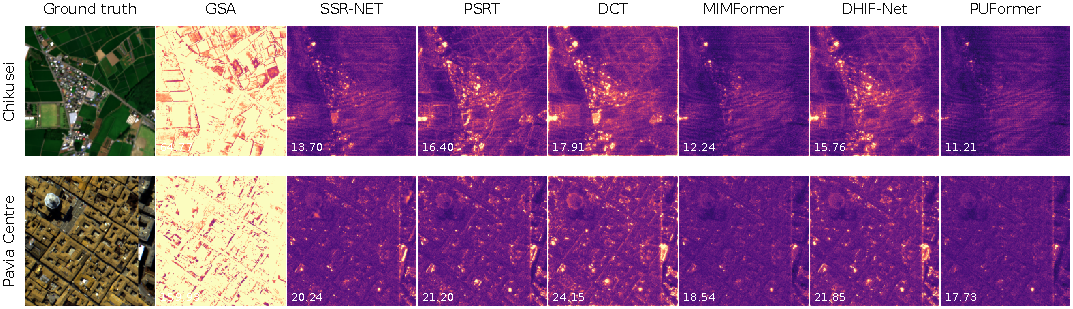
\includegraphics[width=\textwidth]{figures/q1_visual.pdf}
\caption{Mean absolute error over all bands (DN) on the test image where PUFormer has its lowest PSNR. The color scale is set by the retrained networks (clipped at the 99.5th percentile), so GSA saturates; the number in each map is its mean.}
\label{fig:visual}
\end{figure*}}{}

\subsection{Where the margin comes from}
\label{sec:nullsplit}
\qtab{cvpr_margin}

\Cref{tab:margin} reduces PUFormer step by step. A single U-Net prior on the bicubic image and the HR-MSI, without data steps or stages, already reaches \qone{gain-chikusei-abl-unet-psnr}~dB on Chikusei and \qone{gain-pavia-abl-unet-psnr}~dB on Pavia Centre, above every retrained network. Most of the margin therefore comes from this residual multiscale prior and its training recipe, not from the transformer blocks, and the exact data steps add \qone{gain-chikusei-abl-unet-gap} and \qone{gain-pavia-abl-unet-gap}~dB on top.

The null space of \cref{thm:kron}(c) gives a second view. We project the error of every method onto the observed subspace $\mathrm{row}(\D)+\mathrm{row}(\R)$, where it contradicts the observations, and onto the null space, where only a prior can reduce it. Bicubic interpolation and GSA err mostly in the observed subspace: only \qone{null-chikusei-bicubic-share}\% and \qone{null-chikusei-gsa-share}\% of their squared error lies in the null space on Chikusei, so they do not even reproduce their inputs. PUFormer's error in the observed subspace (column Obs.\ of \cref{tab:bench}) is \qone{null-chikusei-obs-ratio} times smaller than MIMFormer's on Chikusei and \qone{null-pavia-obs-ratio} times smaller on Pavia Centre. Removing MIMFormer's observed error alone would raise its PSNR by \qone{null-chikusei-consistency-gain}~dB on Chikusei; the remaining \qone{null-chikusei-prior-gain}~dB of PUFormer's margin come from a better estimate of the null-space part. The exact data steps account for the first part, and the prior for the second.

\subsection{What the exact operator does}
\label{sec:ablation}
\qtab{cvpr_ablation}
\qtab{cvpr_cond}

\Cref{tab:ablation} retrains variants from scratch with the same budget. Without data steps, PSNR drops by \qone{kabl-nophys-absdelta}~dB on Chikusei and \qone{abl-nophys-absdelta}~dB on Pavia Centre, and the agreement with the LR-HSI falls from \qone{kabl-full-consH} to \qone{kabl-nophys-consH}~dB. A zero border or a learned blur and response cost \qone{kabl-zeros-absdelta} and \qone{kabl-learned-absdelta}~dB on Chikusei, and both reproduce the LR-HSI about 3~dB worse, as \cref{thm:mismatch} predicts. Over three seeds the zero border costs \qone{kabl-seed-gain}~dB on Chikusei and \qone{abl-seed-gain}~dB on Pavia Centre, against a seed spread of \qone{kabl-full-std} and \qone{abl-full-std}~dB.

The difference becomes large when the blur changes (\cref{fig:operator}). Given the true blur, the exact model loses at most \qone{kabl-full-swaploss}~dB on Chikusei; the zero-border model, given the same blur, loses \qone{kabl-zeros-swaploss}~dB, and the learned operator, which cannot be replaced, \qone{kabl-learned-fixedloss}~dB. A zero border thus prevents the swap from working although it differs from the exact operator only at the image border: the prior has learned to compensate a border error tied to the training blur. Solving the data step exactly in closed form~\eqref{eq:kronstep} costs little training speed (\qone{kabl-kron-iters} against \qone{kabl-full-iters} iterations on Chikusei), changes the PSNR by \qone{kabl-kron-delta} and \qone{abl-kron-delta}~dB (Chikusei, Pavia Centre) and reproduces the LR-HSI about 3~dB more accurately (\qone{kabl-kron-consH} against \qone{kabl-full-consH}~dB on Chikusei). Learning its spectral gains~\eqref{eq:klstep} changes the PSNR by \qone{kabl-kl-delta} and \qone{abl-kl-delta}~dB and raises this agreement further, to \qone{kabl-kl-consH}~dB. The exact proximal step with five conjugate-gradient iterations is slower and completes fewer training iterations in the budget. Changes to the prior matter less: a convolutional mixer instead of attention changes the PSNR by \qone{kabl-conv-delta} and \qone{abl-conv-delta}~dB (Chikusei, Pavia Centre), and a single stage by \qone{kabl-k1-delta} and \qone{abl-k1-delta}~dB.

\begin{figure}[t]
\centering
\IfFileExists{figures/q1_operator.pdf}{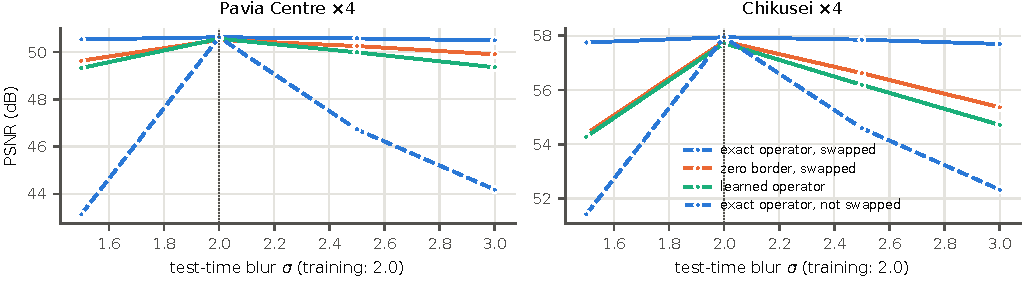
\includegraphics[width=\columnwidth]{figures/q1_operator.pdf}}{}
\caption{Test PSNR when the test blur differs from the training blur ($\sigma_0=2$, dotted): exact operator with and without the true blur, zero border with the true blur, and a learned operator, which cannot be replaced.}
\label{fig:operator}
\end{figure}

\subsection{One network for a family of observation models}
\label{sec:cond}

\Cref{tab:cond} tests networks trained over the operator family on conditions that leave the training protocol. Within the family, the estimate of \cref{thm:ident} is accurate: on every test image and condition, 30~dB SNR included, the blur width is recovered to within \qone{cond-chikusei-sigerr-max} and the spectral shift to within \qone{cond-chikusei-shifterr-max}~nm on Chikusei. Training over the family is what makes the network robust to noise and to combined changes: at 40--30~dB SNR the mean PSNR rises from \qone{cond-chikusei-noise-bench-puformer-fixed} to \qone{cond-chikusei-noise-cond-omc-estimated}~dB on Chikusei. Giving the data steps the estimated operator adds to randomized training alone, \eg \qone{cond-chikusei-combined-cond-omc-estimated} against \qone{cond-chikusei-combined-cond-nocond-fixed}~dB under combined changes, and MIMFormer trained on the same randomized data stays below both. The price is a lower PSNR at the training operator (\qone{cond-chikusei-nominal-cond-omc-estimated} against \qone{chikusei4-psnr}~dB).

Outside the family the operator-conditioned network is fragile. With an anisotropic or defocus blur the estimated isotropic operator is wrong, and the network, which trusts its operator, drops to \qone{cond-chikusei-kernel-cond-omc-estimated}~dB on Chikusei, below the network trained on randomized data with the nominal operator (\qone{cond-chikusei-kernel-cond-nocond-fixed}~dB); given the true kernel it recovers (\qone{cond-chikusei-kernel-cond-omc-oracle}~dB). An HR-MSI misregistered by half a pixel costs every method, GSA included, more than 15~dB, because none of them models registration. Exactness thus makes the network precise when the operator family covers the test conditions and fragile when it does not.

\section{Limitations and conclusion}
\label{sec:conclusion}
Most results rest on Wald's protocol, as in every benchmark of this field. On real airborne NEON data, an imaging spectrometer with a co-registered RGB camera whose response we fit (\supp), PUFormer is again the most accurate at reduced resolution (\qone{neon-puformer-psnr} against \qone{neon-mimformer-psnr}~dB for MIMFormer), but the operator variants differ by less than 0.1~dB there, because the fitted response is only approximate. Real sensor pairs also have registration errors, which our operator family does not cover. The equal-budget benchmark trains every method for 4~h; the 8~h check narrows but keeps the gap, but fully converged comparisons were not run. The test sets of Chikusei and Pavia Centre are small.

We studied exact observation operators in unfolded hyperspectral and multispectral fusion. Separable operators with the true border give a closed-form data step and an explicit null space; an exact data step keeps the ground truth fixed and an inexact one moves it by a bounded amount; and both operators can be estimated from the observations. Under one protocol and budget, PUFormer is more accurate than \qone{n-retrained-word} retrained networks, mainly because of its prior and training, while its exact operators make it adaptable to new blurs, spectral responses and noise. Operator families that include non-separable blurs and registration errors are the next step. Code will be made publicly available.

\section*{LLM Usage Statement}
\TODO{Required by CVPR 2027 (does not count toward the page limit). It must truthfully name any LLM or generative AI tool used for this work, the parts it was used for (e.g., code, experiments, text editing) and the extent of use. Draft to be completed by the authors: ``A large language model assistant was used to help write and debug the training and evaluation code, to run the experiments on cloud GPUs, and to edit the text. The authors designed the study, checked all code, results and claims, and take full responsibility for the content.''}

{
    \small
    \bibliographystyle{ieeenat_fullname}
    \bibliography{references}
}

\end{document}
